\documentclass[a4paper,12pt]{report}
\usepackage[T1]{fontenc}
\usepackage[utf8]{inputenc}
\def\magyarOptions{defaults=hu-min}
\usepackage[magyar]{babel}
\usepackage{amsthm, amssymb, amsmath}
\usepackage[hidelinks]{hyperref}
\usepackage{enumerate, graphicx, xcolor}
\usepackage{booktabs}
\usepackage[htt]{hyphenat}
\usepackage{xurl}
\usepackage{tabularx}
\usepackage{subcaption}
\usepackage{float}
\usepackage{listings}
\usepackage[section]{placeins}
\renewcommand{\lstlistingname}{Kódrészlet}
\lstset{
  language=C,
  basicstyle=\ttfamily\footnotesize,
  commentstyle=\itshape,
  breaklines=true,
  frame=single,
  captionpos=b,
  numbers=left,
  numberstyle=\tiny,
  xleftmargin=1.5em
}

\usepackage{chngcntr}
\counterwithout{figure}{chapter}
\counterwithout{figure}{section}
\counterwithout{figure}{subsection}
\usepackage[nobysame]{amsrefs}

\usepackage{geometry}
 \geometry{
 a4paper,
 total={160mm,247mm},
 left=25mm,
 top=25mm,
 }

\newtheorem{theo}{tétel}[section]
\newtheorem{defin}[theo]{definíció}
\newtheorem{lemma}[theo]{lemma}
\newtheorem{all}[theo]{állítás}
\newtheorem{kov}[theo]{következmény}

\theoremstyle{definition}
\newtheorem{definition}[theo]{definíció}

\theoremstyle{remark}
\newtheorem{megj}[theo]{megjegyzés}

\date{today}
\linespread{1.3}
\frenchspacing
\emergencystretch=2em

\begin{document}
\thispagestyle{empty}

% ============================================================
% CÍMLAP
% ============================================================
\pagenumbering{roman}
\thispagestyle{empty}

\begin{center}
\vspace*{0.2cm} {\Large\bf Szegedi Tudományegyetem}
\vspace{0.3cm}

{\Large\bf Természettudományi és Informatikai Kar}
\vspace{0.3cm}

{\Large\bf Informatikai Intézet}
\vspace{3cm}

{\Large SZAKDOLGOZAT}

\vspace*{1.5cm}

{\LARGE\bf Lightweight kriptográfiai algoritmusok teljesítmény-elemzése erőforrás-korlátozott rendszerekre}

\vspace{0.4cm}
Performance Analysis of Lightweight Cryptographic Algorithms for Resource-Constrained Systems

\vspace*{4cm}

{\large
\begin{tabular}{c@{\hspace{2cm}}c}
\emph{Készítette:}     &\emph{Témavezető:}\\
\bf{Kárász Barna Kristóf}  &\bf{Dr. Békési József}\\
Mérnökinformatikus BSc hallgató    & \\
&
\end{tabular}
}

\vspace*{1.5cm}

{\Large Szeged\\ \vspace{2mm} 2026}
\end{center}

% ============================================================
% KIVONAT
% ============================================================
\begin{abstract}
Az IoT-eszközök jelentős része kevés memóriával, alacsony órajellel és szűkös energiával működő mikrovezérlő, amelyen a megszokott kriptográfiai megoldások futtatása költséges. A dolgozat négy szimmetrikus kriptográfiai algoritmust hasonlít össze egy ARM Cortex-M4 magos STM32L432KC mikrovezérlőn: az AES-128-at mint viszonyítási alapot, a SPECK~128/128 és a LEA-128 könnyűsúlyú blokktitkosítót, valamint az Ascon v1.2 szerinti ASCON-128 hitelesített titkosítási sémát; a NIST 2025-ös szabványa (SP~800-232) ugyanennek a családnak a 128a változatára épül. Az algoritmusokat a publikált specifikációk és referenciakódok alapján egységes, tesztvektorokkal ellenőrzött C-implementációkban valósítottuk meg, és a processzormag ciklusszámlálójával mértük a kulcsgenerálás, a titkosítás és a visszafejtés költségét 16 és 1024 bájt közötti üzenetméreteken, hat fordítói optimalizációs szinten. A mért ciklusszámokból a fajlagos költséget és a feldolgozási sebességet is meghatároztuk, emellett a kódméretet és a veremigényt is vizsgáltuk. \texttt{-O3} optimalizáció mellett az ARX-alapú SPECK és LEA a vizsgált AES-implementációnál titkosításkor 3,7--4,5-ször, visszafejtéskor 8,7--10-szer kisebb fajlagos költséggel dolgozott. Az ASCON-128 a hitelesítéssel együtt is gyorsabb volt a hitelesítést nem végző AES-nél, ha az üzenet kb.\ 80 bájtnál hosszabb volt; méretre optimalizált fordításnál ez a határ kb.\ 23 bájtra csökkent. Az algoritmusok biztonsági jellemzőit a szakirodalom alapján foglaljuk össze, végül a mérések alapján alkalmazási ajánlásokat fogalmazunk meg.

{\bf Kulcsszavak:} könnyűsúlyú kriptográfia, IoT-biztonság, blokktitkosító, AES, SPECK, LEA, ASCON, Cortex-M4, teljesítménymérés
\end{abstract}

\newpage
\pagebreak
\tableofcontents
\pagebreak

% ============================================================
% 1. FEJEZET – BEVEZETÉS
% ============================================================
\pagenumbering{arabic}
\chapter{Bevezetés}

Az elmúlt évtizedben a hálózatba kapcsolt eszközök az ipar, a közlekedés és a háztartások mindennapi részévé váltak. Az \emph{Ipar 4.0} keretében a gyártósorok, a logisztikai láncok és az épületgépészeti rendszerek egyre inkább egymással kommunikáló eszközökre épülnek \cite{Sadeghi2015}. A dolgok internete (Internet of Things, IoT) ma már nem csupán kutatási téma: okos termosztátok, viselhető egészségügyi eszközök, mezőgazdasági szenzorok és közlekedésirányító rendszerek alkotják.

Az Ericsson jelentése szerint 2025 végén világszerte 22,3 milliárd IoT-kapcsolat volt, és ez a szám 2031-re megközelítheti a 47,1 milliárdot \cite{Ericsson2026}. Ezeknek az eszközöknek jelentős része nem számítógép vagy okostelefon, hanem mikrovezérlő, szenzor vagy RFID-címke, amely kevés memóriával, alacsony órajellel és szűkös, gyakran elemről biztosított energiaellátással működik.

Ezek az eszközök sokszor érzékeny adatokat kezelnek. Egy gyártósoron a meghamisított szenzorérték vagy vezérlőparancs anyagi és fizikai kárt okozhat, egy közlekedési rendszerben a módosított adat balesethez vezethet, egy egészségügyi eszköznél pedig a kiszivárgó betegadat súlyos adatvédelmi következményekkel jár. A kommunikáció titkosítása és hitelesítése ezért ezeken az eszközökön is alapkövetelmény \cite{Hossain2015}.

A széles körben használt kriptográfiai eljárásokat nem elsősorban ilyen eszközökre tervezték. Az aszimmetrikus algoritmusok (pl.~RSA) egy kis mikrovezérlőn lassúak és sok energiát fogyasztanak, de még a szimmetrikus AES is érezhető részt foglalhat el a legszűkebb eszközök memóriájából és számítási idejéből. Erre a problémára kínál megoldást a \emph{könnyűsúlyú} (lightweight) \emph{kriptográfia}, amely kevés erőforrással is az adott alkalmazáshoz elegendő biztonságot igyekszik nyújtani \cite{NISTIR8114}.

A terület jelentőségét jól mutatja, hogy a NIST (National Institute of Standards and Technology) 2018-ban külön szabványosítási eljárást indított a könnyűsúlyú kriptográfiára, és 2023-ban a grazi kutatók által tervezett ASCON-t választotta ki szabványnak \cite{NISTLWC2023}.

\bigskip

A dolgozatban négy, eltérő felépítésű kriptográfiai algoritmust hasonlítunk össze. Célunk annak megmérése, hogy az egyes algoritmusok mekkora futásidejű költséggel járnak egy erőforrás-korlátozott eszközön. A méréseket egy ARM Cortex-M4 magos STM32L432KC mikrovezérlőn végeztük: a kulcsgenerálás, a titkosítás és a visszafejtés ciklusszámát mértük, ebből pedig a fajlagos költséget és a feldolgozási sebességet határoztuk meg, hat fordítói optimalizációs szinten. A vizsgált algoritmusok:

\begin{enumerate}
	\item \textbf{AES-128} -- az iparban legelterjedtebb szimmetrikus blokktitkosító, amely az összehasonlításban viszonyítási alapként szolgál;
	\item \textbf{SPECK~128/128} -- az NSA által tervezett, szoftveres futásra optimalizált, ARX-alapú könnyűsúlyú blokktitkosító;
	\item \textbf{LEA-128} -- a dél-koreai NSRI által kidolgozott könnyűsúlyú blokktitkosító, amely az ISO/IEC 29192-2:2019 szabvány része;
	\item \textbf{ASCON-128} -- a NIST által 2023-ban kiválasztott ASCON család szivacskonstrukcióra épülő hitelesített titkosítási sémája (az Ascon v1.2 specifikáció szerinti változat).
\end{enumerate}

Az algoritmusokat úgy választottuk ki, hogy mindegyik más tervezési elvet képviseljen (SPN, ARX-alapú Feistel-hálózat, ARX-alapú általánosított Feistel-hálózat, illetve szivacskonstrukció), ugyanakkor összevethetők maradjanak: mind a négy 128 bites kulcsot használ, a blokktitkosítók 128 bites blokkot, és mindegyik jól megvalósítható szoftverben. Így a mért különbségeket nemcsak közölni, hanem az algoritmusok felépítésével magyarázni is tudjuk.

A dolgozat felépítése a következő. A~\ref{chap:hatter}.~fejezet a szimmetrikus kriptográfia alapjait, a hashfüggvényeket és az üzenethitelesítést, az erőforrás-korlátozott rendszerek jellemzőit, valamint a könnyűsúlyú kriptográfia megjelenésének okait mutatja be. A~\ref{chap:algoritmusok}.~fejezet a négy kiválasztott algoritmust ismerteti és veti össze. A~\ref{chap:implementacio}.~fejezet a szoftveres megvalósítást és a mérési módszert, az~\ref{chap:meresek}.~fejezet a mérési eredményeket tárgyalja. A~\ref{chap:biztonsag}.~fejezet a szakirodalom alapján összeveti az algoritmusok biztonsági jellemzőit, végül a~\ref{chap:osszefoglalas}.~fejezet összegzi az eredményeket, alkalmazási ajánlásokat fogalmaz meg, és továbbfejlesztési lehetőségeket vázol fel.

% ============================================================
% 2. FEJEZET – HÁTTÉRISMERETEK
% ============================================================
\chapter{Háttérismeretek}\label{chap:hatter}

Ez a fejezet azokat az alapokat foglalja össze, amelyekre a dolgozat további része épül: a szimmetrikus kriptográfia fő fogalmait, a hashfüggvényeket és az üzenethitelesítést, az erőforrás-korlátozott eszközök jellemzőit, valamint azokat a gyakorlati okokat, amelyek miatt a könnyűsúlyú kriptográfia önálló kutatási területté vált.

% -------------------------------------------------------
\section{Szimmetrikus kriptográfia alapjai}\label{sec:szimmetrikus}
% -------------------------------------------------------

A \emph{szimmetrikus kriptográfiában} a titkosítás és a visszafejtés \emph{ugyanazzal a titkos kulccsal} történik. Formálisan: adott egy $E$ titkosító és egy $D$ visszafejtő függvény, amelyekre tetszőleges $P$ nyílt szöveg és $K$ kulcs esetén $D(K, E(K, P)) = P$ \cite{Stallings2017}. Az aszimmetrikus (nyilvános kulcsú) eljárásoknál lényegesen kevesebb számítást igényelnek, ezért erőforrás-korlátozott eszközökön elsősorban ezeket használják az adatok titkosítására.

\subsection{Blokktitkosítók}

A szimmetrikus titkosítás leggyakoribb formája a \emph{blokktitkosító} (block cipher). Ez a bemenetet rögzített méretű, jellemzően 64 vagy 128 bites egységekre, úgynevezett \emph{blokkokra} bontja, és mindegyiket a kulcs függvényében egy azonos méretű titkosított blokká alakítja \cite{Paar2010}. A blokktitkosító több \emph{körből} (round) áll. Egy-egy kör önmagában egyszerű műveleteket végez, de kellő számú ismétlés után a kimenet már nem mutat kihasználható összefüggést a bemenettel és a kulccsal. A tervezés két alapelvét Claude Shannon fogalmazta meg 1949-ben~\cite{Shannon1949}:

\begin{itemize}
	\item \textbf{Konfúzió} (confusion): a titkosított szöveg és a kulcs közötti kapcsolatnak a lehető legbonyolultabbnak kell lennie. Ezt nemlineáris műveletek biztosítják, például helyettesítő táblák (S-boxok) vagy moduláris összeadás.
	\item \textbf{Diffúzió} (diffusion): a nyílt szöveg egyetlen bitjének megváltozása a titkosított szöveg minél több bitjére hasson ki. Ezt permutációk, bitforgatások vagy lineáris transzformációk (pl.~véges test feletti mátrixszorzás) érik el.
\end{itemize}

A következőkben a blokktitkosítók három gyakori felépítését mutatjuk be. A dolgozatban vizsgált blokktitkosítók mindegyike ezek valamelyikére épül.

\subsubsection{SPN -- helyettesítő-permutációs hálózat}

A \emph{Substitution-Permutation Network} (SPN) felépítésű blokktitkosítók minden körben három réteget alkalmaznak. A \emph{helyettesítő réteg} (substitution layer) a blokkot kisebb, általában 4 vagy 8 bites részekre bontja, és mindegyiket egy rögzített nemlineáris leképezésen, az \emph{S-boxon} vezeti át. Az S-box felel elsősorban a konfúzióért.

A második, \emph{diffúziós réteg} szétteríti az S-boxok kimenetét a blokkon, így a következő körben minden S-box több előző S-box eredményét kapja meg. Egyszerűbb SPN-eknél ez a bitek átrendezése (permutációja), az AES-nél viszont egy lineáris transzformáció (ShiftRows és MixColumns). Néhány kör után így a nyílt szöveg egyetlen bitjének változása a teljes kimeneti blokkot érinti. Végül a \emph{körkulcs hozzáadása} (round key addition) során egy XOR művelet keveri az állapotba a fő kulcsból származtatott körkulcsot. Az SPN legismertebb képviselője az AES \cite{DaemenRijmen2002}.

\subsubsection{Feistel-hálózat}

A Horst Feistelről elnevezett szerkezet a blokkot két egyenlő félre, $L$-re (bal) és $R$-re (jobb) bontja. Minden körben az $R$ félre egy $F$ körfüggvényt alkalmaz az aktuális körkulccsal, az eredményt XOR-ral hozzáadja az $L$ félhez, majd a két felet felcseréli:
\begin{align}
	L_{i+1} &= R_i, \nonumber\\
	R_{i+1} &= L_i \oplus F(R_i, K_i).
\end{align}
A Feistel-hálózat nagy előnye, hogy a visszafejtés ugyanazzal a szerkezettel történik, mint a titkosítás, csak a körkulcsokat kell fordított sorrendben alkalmazni. Ezért az $F$ függvénynek nem kell invertálhatónak lennie \cite{Paar2010}. A szerkezet legismertebb példája a DES (Data Encryption Standard), amelynek 16 körös Feistel-hálózata 1977-től évtizedekig meghatározó szabvány volt. 56 bites kulcsa azonban ma már nem véd a kulcstér végigpróbálása (brute force) ellen.

\subsubsection{ARX-szerkezet}

Az \emph{Add-Rotate-XOR} (ARX) megközelítés három egyszerű műveletre épül \cite{Beaulieu2013}:

\begin{itemize}
	\item \textbf{Add} -- moduláris összeadás ($\bmod 2^n$): az átvitelek terjedése miatt ez a nemlineáris elem, amely S-box nélkül biztosítja a konfúziót;
	\item \textbf{Rotate} -- bitforgatás (ciklikus eltolás): a szón belüli diffúziót szolgálja;
	\item \textbf{XOR} -- kizáró vagy: a körkulcs bekeverésére és az ágak összekeverésére szolgál.
\end{itemize}

Az ARX fő előnye az egyszerűség. Ha a szóméret megegyezik a processzor regiszterszélességével, mindhárom művelet egyetlen gépi utasítás, és nincs szükség memóriában tárolt helyettesítő táblára. Mivel a műveletek végrehajtási ideje nem függ a feldolgozott adattól, az ARX-algoritmusok könnyen megvalósíthatók \emph{konstans idejű} (constant-time) kóddal, ami fontos védelem az időzítéses oldalcsatorna-támadások (timing attacks) ellen. A dolgozatban vizsgált SPECK és LEA egyaránt ARX-alapú, de eltérő szerkezetben használja ezeket a műveleteket.

\subsection{Üzemmódok}\label{sec:uzemmodok}

A blokktitkosító egyszerre csak egy rögzített méretű blokkot dolgoz fel, a valódi üzenetek hossza viszont tetszőleges. Azt, hogy az egymást követő blokkokat hogyan titkosítjuk és hogyan kapcsoljuk össze, az \emph{üzemmód} (mode of operation) határozza meg. A legfontosabbak \cite{Stallings2017}:

\begin{itemize}
	\item \textbf{ECB} (Electronic Codebook): minden blokkot egymástól függetlenül, ugyanazzal a kulccsal titkosítunk. Egyszerű és párhuzamosítható, de az azonos nyíltszöveg-blokkokból mindig azonos titkosított blokkok lesznek, így az adat mintázatai (például egy kép körvonalai) a titkosított szövegben is látszanak. Ezért önmagában nem ajánlott.
	\item \textbf{CBC} (Cipher Block Chaining): titkosítás előtt minden nyíltszöveg-blokkot XOR-ral összekapcsolunk az \emph{előző} titkosított blokkal; az első blokkhoz egy véletlenszerű inicializációs vektort (IV) használunk. A láncolás miatt azonos bemeneti blokkokból különböző kimenet keletkezik. Hátránya, hogy a titkosítás nem párhuzamosítható.
	\item \textbf{CTR} (Counter Mode): a blokktitkosító egy minden blokknál más számlálóértéket titkosít, és az így kapott \emph{kulcsfolyamot} (keystream) XOR-ral adjuk a nyílt szöveghez. A számlálóértékek előre ismertek, ezért a titkosítás és a visszafejtés is párhuzamosítható, a visszafejtéshez pedig elég a titkosító függvény. Lényeges feltétel, hogy ugyanazzal a kulccsal egy számlálóérték soha ne ismétlődjön.
\end{itemize}

\subsection{A DES és az AES rövid áttekintése}

A \emph{Data Encryption Standard} (DES) az 1977-es szabványosítás után évtizedekig a legszélesebb körben használt szimmetrikus algoritmus volt. Feistel-hálózata 16 körből áll, a nemlineáris lépést 8 darab, 6 bites bemenetet 4 bites kimenetre képező S-box végzi. A szabvány bukását az 56 bites kulcs okozta: 1998-ban az Electronic Frontier Foundation (EFF) erre a célra épített gépe 56 óra alatt találta meg a kulcsot, 1999-ben pedig a distributed.net önkéntes hálózatával közösen alig több mint 22 óra alatt \cite{Paar2010}. A Triple-DES (3DES) ideiglenesen megoldotta a kulcsméret problémáját, de lassú volt, és 64 bites blokkmérete is korlátot jelentett, ezért új szabványra volt szükség.

Az \emph{Advanced Encryption Standard} (AES) 2001-ben váltotta fel a DES-t. A NIST nyílt pályázatát a belga Joan Daemen és Vincent Rijmen Rijndael nevű algoritmusa nyerte meg \cite{FIPS197}. Az AES SPN-szerkezetű, 128 bites blokkokkal dolgozik, kulcsa 128, 192 vagy 256 bites, amelyekhez rendre 10, 12 és 14 kör tartozik. Ma az AES a szimmetrikus kriptográfia etalonja: számos processzor hardveresen gyorsítja (pl.~az Intel AES-NI utasításkészlettel), és a teljes algoritmus ellen nem ismert gyakorlatban kivitelezhető támadás. Ezért szolgál az AES-128 a dolgozatban viszonyítási alapként: azt vizsgáljuk, mennyi erőforrást takaríthatnak meg hozzá képest a könnyűsúlyú algoritmusok, és ennek milyen biztonsági ára van.

% -------------------------------------------------------
\section{Hashfüggvények és üzenethitelesítés}\label{sec:hash}
% -------------------------------------------------------

A biztonságos kommunikációhoz a titkosság mellett \emph{integritás} (az adat sértetlensége) és \emph{hitelesség} (a feladó igazolása) is szükséges \cite{Stallings2017}. Ezeket kriptográfiai hashfüggvényekkel, üzenethitelesítő kódokkal (MAC) és hitelesített titkosítási sémákkal (AEAD) lehet biztosítani.

\subsection{Kriptográfiai hashfüggvények}

A hashfüggvény tetszőleges hosszúságú bemenetből rögzített méretű kimenetet, \emph{lenyomatot} (digest) állít elő. Biztonsági célra akkor alkalmas, ha teljesíti a következő három feltételt \cite{Paar2010}:
\begin{enumerate}
	\item \textbf{Egyirányúság} (preimage resistance): a lenyomatból gyakorlatilag ne lehessen olyan bemenetet találni, amely ezt a lenyomatot adja.
	\item \textbf{Második ősképpel szembeni ellenállás} (second preimage resistance): egy adott bemenethez ne lehessen olyan másik bemenetet találni, amelynek ugyanaz a lenyomata.
	\item \textbf{Ütközésállóság} (collision resistance): ne lehessen hatékonyan találni két tetszőleges, különböző bemenetet azonos lenyomattal.
\end{enumerate}
Ma a SHA-2 és a SHA-3 család a szabványos választás; az MD5 és a SHA-1 a megtalált ütközések miatt biztonsági célra már nem használható.

\subsection{MAC -- üzenethitelesítő kód}

A MAC (Message Authentication Code) előállításához egy közös titkos kulcs is kell, ezért az integritás mellett a hitelességet is biztosítja: érvényes MAC-ot csak az tud előállítani, aki ismeri a kulcsot. A két legelterjedtebb változat a hashfüggvényre épülő HMAC \cite{Stallings2017} és a blokktitkosítót láncolva használó CBC-MAC.

\subsection{AEAD -- hitelesített titkosítás kapcsolódó adatokkal}\label{sec:aead}

A gyakorlat azt mutatta, hogy a titkosítást és a hitelesítést célszerű egyetlen, együtt tervezett eljárásban elvégezni. Ezt valósítják meg az AEAD (Authenticated Encryption with Associated Data) sémák \cite{Dobraunig2021}. Bemenetük a titkos kulcs, egy csak egyszer használható érték (nonce), a nyílt szöveg és a \emph{kapcsolódó adat} (associated data, AD). Ez utóbbi, például egy hálózati csomag fejléce, titkosítatlan marad, hogy a hálózati eszközök olvashassák, de a séma hitelesíti, így módosítása kiderül.

A kimenet a titkosított szöveg és egy \emph{hitelesítő címke} (tag), amely a titkosított szöveg és a kapcsolódó adat sértetlenségét igazolja. Az AEAD sémák egyik legfontosabb feltétele, hogy ugyanazzal a kulccsal egy nonce-ot ne használjunk kétszer, mert ez a legtöbb sémánál súlyosan sérti a biztonságot. A dolgozat szempontjából azért fontos az AEAD, mert az ASCON a többi vizsgált algoritmussal ellentétben nem blokktitkosító, hanem eleve ilyen sémának készült.

% -------------------------------------------------------
\section{Erőforrás-korlátozott rendszerek jellemzői}\label{sec:eroforras}
% -------------------------------------------------------

A könnyűsúlyú kriptográfia célpontjai jellemzően kis teljesítményű, kevés memóriával és szűkös energiával rendelkező eszközök.

\subsection{Mikrovezérlők és erőforrásaik}\label{sec:mikrovezerlok}

Az IoT-eszközökben használt processzorok szóméretük szerint három fő csoportba sorolhatók:
\begin{itemize}
	\item \textbf{8 bites} (pl.~ATmega): néhány MHz-es órajel, néhány kilobájt RAM. Egyszerű szenzorokban és beágyazott vezérlőkben gyakoriak.
	\item \textbf{16 bites} (pl.~MSP430): nagyon alacsony fogyasztásra tervezett platformok, amelyeket gyakran használnak vezeték nélküli szenzorhálózatokban (WSN) \cite{NISTIR8114}.
	\item \textbf{32 bites} (pl.~ARM Cortex-M, ESP32): ipari átjárókban és összetettebb szenzorrendszerekben használt eszközök, akár megabájtos flash-memóriával, de még így is nagyságrendekkel kisebb kapacitással, mint egy asztali számítógép.
\end{itemize}

Ezek a korlátok közvetlenül meghatározzák, milyen kriptográfiai megoldás futtatható az eszközön. A programkód és a konstansok a flash-memóriában, a változók és a körkulcsok a jellemzően sokkal kisebb RAM-ban kapnak helyet; egy RFID-címkén például mindössze 300--500 bájt RAM állhat rendelkezésre \cite{Hatzivasilis2018}. Sok kis processzorból hiányzik a hardveres szorzó vagy a kriptográfiai gyorsító, így minden műveletet egyszerű utasításokból kell felépíteni. Elemes eszközöknél minden elvégzett óraciklus energiát fogyaszt, ezért a kriptográfiai műveletek költsége is befolyásolja, meddig működik az eszköz egy töltéssel vagy elemcserével \cite{NISTIR8114}.

Ilyen eszközök működnek többek között az ipari rendszerekben (például PLC-k és SCADA-rendszerek környezetében) \cite{Sadeghi2015}, az okosváros-infrastruktúrában és az egészségügyi eszközökben, ahol egyszerre van szükség erős adatvédelemre és takarékos működésre. Ezeken a területeken válik igazán fontossá a könnyűsúlyú kriptográfia.

% -------------------------------------------------------
\section{A lightweight kriptográfia motivációja}\label{sec:lwc_motivacio}
% -------------------------------------------------------

\subsection{A hagyományos szabványok korlátai}

Az AES-t kifejezetten úgy tervezték, hogy sokféle platformon, a 8 bites smart cardoktól a szerverekig hatékonyan fusson \cite{DaemenRijmen2002}. A legszűkebb eszközökön azonban így is jelentős a költsége: a 256 bájtos S-box tábla a néhány kilobájtos memóriából érezhető részt foglal el, a véges test feletti MixColumns lépés pedig 8 bites processzoron sok utasítást igényel. Hardveres megvalósítása nagyjából 2400 kapuegyenértéknyi (gate equivalent, GE) területet foglal, ami a legolcsóbb RFID-chipeken túl sok \cite{NISTIR8114}.

A könnyűsúlyú kriptográfia ezért a szűkös erőforrások és az elvárt biztonság közötti egyensúlyt keresi. Egy IoT-eszköz általában nem igényel 256 bites biztonsági szintet; a 128 bites szint a jelenlegi ismeretek szerint az eszköz teljes élettartamára elegendő védelmet nyújt \cite{Biryukov2017}. A cél tehát az, hogy ez a biztonsági szint a lehető legkevesebb memóriával és energiával legyen elérhető, például kisebb S-boxokkal vagy egyszerű ARX-műveletekkel.

\subsection{A NIST Lightweight Cryptography szabványosítás}

A NIST 2018-ban hirdetett nyílt pályázatot erőforrás-korlátozott eszközökre szánt hitelesített titkosítási (AEAD) sémák szabványosítására \cite{NISTLWC2023}. A jelöltek kulcsa legalább 128 bites lehetett, és a kriptoanalitikai támadásoknak legalább $2^{112}$ műveletet kellett igényelniük, a meglévő NIST-szabványoknál lényegesen jobb hatékonyság mellett.

A beérkezett 57 pályázatból 56 jutott az első fordulóba, 2021-ben tíz döntős maradt, és 2023 februárjában a NIST az \emph{ASCON}-t választotta ki. A döntésben szerepet játszott, hogy az ASCON egyetlen, 320 bites állapoton dolgozó permutációra épül, amelyet szivacs- (duplex-) konstrukcióban használ, így egyszerűen és hatékonyan megvalósítható hardverben és szoftverben is \cite{Dobraunig2021}. A végleges szabvány NIST SP~800-232 néven 2025-ben jelent meg~\cite{NISTSP800232}.

% ============================================================
% 3. FEJEZET – VIZSGÁLT ALGORITMUSOK
% ============================================================
\chapter{Vizsgált algoritmusok bemutatása}\label{chap:algoritmusok}

Ez a fejezet a négy vizsgált algoritmus felépítését, kulcsgenerálását és azokat a tulajdonságait mutatja be, amelyekre a mérési eredmények értelmezésénél támaszkodunk.

% -------------------------------------------------------
\section{AES-128}\label{sec:aes}
% -------------------------------------------------------

Az AES eredeti neve \emph{Rijndael}, amely a két belga tervező, Joan Daemen és Vincent Rijmen nevéből állt össze. A NIST 1997-ben kiírt pályázatára 15 jelölt érkezett; a Rijndael a biztonsága, a hatékonysága és a sokféle platformon való jó megvalósíthatósága miatt nyert, és 2001-ben FIPS~197 néven szabvány lett \cite{FIPS197,DaemenRijmen2002}.

\subsection{Felépítés és működés}\label{sec:aes_struktura}

Az AES-128 SPN-szerkezetű blokktitkosító: 128 bites blokkokat dolgoz fel 128 bites kulccsal, 10 körben. A belső állapot (\emph{State}) egy $4 \times 4$-es bájtmátrix. Egy kör négy lépésből áll:

\begin{enumerate}
	\item \textbf{SubBytes} -- minden bájtot egy 256 elemű S-boxon vezet át. Az S-box a $GF(2^8)$ feletti multiplikatív inverzen és egy affin transzformáción alapul, ez adja a konfúziót.
	\item \textbf{ShiftRows} -- a mátrix $i$-edik sorát $i$ pozícióval balra forgatja, így egy oszlop bájtjai a következő lépésben különböző oszlopokba kerülnek.
	\item \textbf{MixColumns} -- minden oszlopot egy rögzített mátrixszal szoroz $GF(2^8)$ felett, így egy bemeneti bájt az oszlop mind a négy kimeneti bájtjára hat. Az utolsó körből ez a lépés kimarad.
	\item \textbf{AddRoundKey} -- XOR-ral hozzáadja az állapothoz az aktuális körkulcsot.
\end{enumerate}

A visszafejtés ezek inverzeit alkalmazza fordított sorrendben. A titkosító MixColumns együtthatói kicsik (1, 2, 3), ezért a szorzás egy-egy kettővel való szorzásra (\emph{xtime}) és XOR-ra vezethető vissza. Az inverz MixColumns együtthatói (9, 11, 13, 14) viszont nagyobbak, így szoftverben lényegesen több műveletet igényel. Ennek a mérésekben is jól látható következménye lesz (\ref{sec:aszimmetria}.~alfejezet).

\subsection{Kulcsgenerálás}\label{sec:aes_kulcs}

Az AES-128 kulcsgenerálása a 128 bites fő kulcsból 11 darab 128 bites körkulcsot (összesen 176 bájtot) állít elő; az első körkulcs maga a fő kulcs. Egy új körkulcs első oszlopához az előző körkulcs utolsó oszlopát egy bájttal elforgatjuk, bájtjait átvezetjük az S-boxon, hozzáadjuk a körkonstanst (Rcon), végül XOR-ral összekeverjük az előző körkulcs első oszlopával. A további oszlopok az előző oszlop és az előző körkulcs megfelelő oszlopának XOR-jaként adódnak \cite{DaemenRijmen2002}.

\subsection{Az AES-128 mint viszonyítási alap}

Az AES-128 a dolgozatban nem könnyűsúlyú algoritmusként, hanem viszonyítási alapként szerepel, mert a legtöbb mai protokoll (TLS, VPN, banki rendszerek) erre épül. Korlátozott eszközökön a 256 bájtos S-box (és visszafejtéshez az inverze) tárolása, valamint a $GF(2^8)$ feletti aritmetika jelent többletköltséget. A vizsgált STM32L432KC-n nincs hardveres AES-gyorsító, így az algoritmus tisztán szoftveresen fut.

% -------------------------------------------------------
\section{SPECK~128/128}\label{sec:speck}
% -------------------------------------------------------

A SPECK algoritmuscsaládot az amerikai Nemzetbiztonsági Ügynökség (NSA) tette közzé 2013-ban, a SIMON családdal együtt \cite{Beaulieu2013}. A SIMON elsősorban hardveres, a SPECK szoftveres megvalósításra készült. A családban több blokk- és kulcsméret is szerepel; mi a 128 bites blokkot és 128 bites kulcsot használó SPECK~128/128 változatot vizsgáljuk.

\subsection{Körfüggvény}\label{sec:speck_kor}

A SPECK~128/128 állapota két 64 bites szó ($x$, $y$). A titkosítás 32 körből áll, minden kör a következő ARX-lépést hajtja végre:
\begin{align}
x &\leftarrow ((x \ggg 8) \mathbin{\boxplus} y) \oplus K_i, \label{eq:speck_round1}\\
y &\leftarrow (y \lll 3) \oplus x, \label{eq:speck_round2}
\end{align}
ahol $\ggg$ és $\lll$ a jobbra, illetve balra forgatás, $\boxplus$ az összeadás $\bmod 2^{64}$, $K_i$ pedig az $i$-edik körkulcs. Egy kör tehát két forgatás, egy összeadás és két XOR; a nemlinearitást egyedül a moduláris összeadás adja \cite{Beaulieu2013}. Visszafejtéskor ugyanezek a lépések fordított sorrendben, kivonással és ellentétes irányú forgatással futnak.

\subsection{Kulcsgenerálás}\label{sec:speck_kulcs}

A kulcsgenerálás ugyanazt a körfüggvényt használja, mint a titkosítás, csak a kör sorszáma tölti be a kulcs szerepét. A 128 bites kulcs két 64 bites szóra bomlik: $K = (l_0, k_0)$, ahol $k_0$ az első körkulcs. A további körkulcsok:
\begin{align}
l_{i+1} &= (k_i \mathbin{\boxplus} (l_i \ggg 8)) \oplus i, \\
k_{i+1} &= (k_i \lll 3) \oplus l_{i+1}.
\end{align}
Ennek két előnye van: a kulcsgeneráláshoz nem kell külön kód, és a körkulcsok menet közben (on the fly) is előállíthatók, nem kell mindet előre a RAM-ban tárolni.

\subsection{Szoftveres megvalósítás}

A SPECK nem használ táblát, végrehajtási ideje nem függ az adattól, és egy 64 bites processzoron minden művelete egyetlen utasítás. Egy 32 bites Cortex-M magon viszont a 64 bites szavakat regiszterpárokban kell kezelni: az összeadás két utasítás (ADDS és ADC), a 64 bites forgatás pedig több eltolásból és kombinálásból áll. Dinu és munkatársai összehasonlító mérésében a SPECK így is a leggyorsabb szoftveres könnyűsúlyú blokktitkosítók közé tartozott \cite{Dinu2015}.

\subsection{Bizalmi kérdések}

A SPECK körüli viták elsősorban nem kriptoanalitikai, hanem bizalmi jellegűek. Az eredeti publikáció nem indokolta részletesen a tervezési döntéseket, például a forgatási paraméterek és a körszám megválasztását; ezt a tervezők 2017-ben részben pótolták \cite{Beaulieu2017}. A SIMON és a SPECK felvételét a könnyűsúlyú blokktitkosítókat tartalmazó ISO/IEC~29192-2 szabványba 2015-ben javasolták, de 2018 áprilisában elutasították, amiben a tervezővel szembeni bizalmatlanság is szerepet játszott \cite{Ashur2021}. Szűkebb területen, az RFID-eszközök légi interfészének kriptográfiai csomagjaként viszont mindkettő ISO/IEC-szabvány lett: az ISO/IEC~29167-21 (SIMON) és a 29167-22 (SPECK) első kiadása 2018-ban jelent meg, a jelenleg érvényes második kiadásuk 2026-ban \cite{ISO29167SIMON,ISO29167}. A nyilvános kriptoanalízis ugyanakkor több mint egy évtized alatt sem talált a teljes körszámú változat ellen gyakorlatban kivitelezhető támadást (\ref{sec:alg_security}.~alfejezet).

% -------------------------------------------------------
\section{LEA-128}\label{sec:lea}
% -------------------------------------------------------

A \emph{Lightweight Encryption Algorithm} (LEA) a dél-koreai Nemzeti Biztonsági Kutatóintézet (NSRI) fejlesztése, amelyet Hong és munkatársai 2013-ban mutattak be \cite{Hong2013}. Elsősorban általános célú, 32 bites processzorokon való gyors szoftveres futásra tervezték. 2019 óta az ISO/IEC~29192-2 szabvány része \cite{ISO29192}, Dél-Koreában pedig a KCMVP (Korean Cryptographic Module Validation Program) által jóváhagyott algoritmus.

\subsection{Általánosított Feistel-hálózat}\label{sec:lea_kor}

A LEA az ARX-műveleteket általánosított Feistel-hálózatban (Generalized Feistel Network, GFN) használja: a 128 bites blokkot négy 32 bites szóra bontja, $(X_0, X_1, X_2, X_3)$. Egy kör \cite{Hong2013}:
\begin{align}
X_0' &= \text{ROL}\big((X_0 \oplus RK_0) \mathbin{\boxplus} (X_1 \oplus RK_1),\; 9\big), \\
X_1' &= \text{ROR}\big((X_1 \oplus RK_2) \mathbin{\boxplus} (X_2 \oplus RK_3),\; 5\big), \\
X_2' &= \text{ROR}\big((X_2 \oplus RK_4) \mathbin{\boxplus} (X_3 \oplus RK_5),\; 3\big), \\
X_3' &= X_0,
\end{align}
ahol $RK_0, \ldots, RK_5$ a kör hat 32 bites körkulcsszava, $\boxplus$ az összeadás $\bmod 2^{32}$, ROL és ROR pedig a balra, illetve jobbra forgatás. A LEA-128 24 körből áll, így összesen $24 \times 6 = 144$ körkulcsszót használ.

\subsection{A 32 bites szóméret}

A LEA és a SPECK legfontosabb gyakorlati különbsége a szóméret. A LEA minden művelete 32 bites, így egy 32 bites magon mindegyik egyetlen utasítás, a forgatás pedig a Cortex-M4 eltolóegysége (barrel shifter) miatt akár egy másik utasításba is beolvasztható. A SPECK~128/128 64 bites szavait ugyanezen a magon csak több utasítással lehet kezelni. A tervezők ezért a LEA-t 32 bites platformokon a SPECK-nél gyorsabbnak várták \cite{Hong2013}; hogy ez a mi méréseinkben mennyiben igazolódott, azt az~\ref{chap:meresek}.~fejezet mutatja meg.

\subsection{Kulcsgenerálás}\label{sec:lea_kulcs}

A LEA-128 kulcsgenerálása négy 32 bites konstansra ($\delta_0, \ldots, \delta_3$) épül, amelyek a $\sqrt{766965}$ hexadecimális kifejtéséből származnak (766965 a „LEA'' betűinek ASCII-kódja). A fő kulcs négy szava $K_0, \ldots, K_3$; az $i$-edik körben
\begin{align}
T_j &= \text{ROL}\big(T_j \mathbin{\boxplus} \text{ROL}(\delta_{i \bmod 4},\; i+j),\; r_j\big), \quad j = 0,1,2,3,
\end{align}
ahol kezdetben $T_j = K_j$, a forgatási paraméterek pedig $r_0 = 1$, $r_1 = 3$, $r_2 = 6$, $r_3 = 11$. A kör hat körkulcsszava $RK = (T_0, T_1, T_2, T_1, T_3, T_1)$. A kulcsgenerálás tehát szintén ARX-műveletekből áll, és menet közben is végrehajtható \cite{Hong2013}.

% -------------------------------------------------------
\section{ASCON-128}\label{sec:ascon}
% -------------------------------------------------------

Az ASCON-t a Grazi Műszaki Egyetem kutatói, Christoph Dobraunig, Maria Eichlseder, Florian Mendel és Martin Schläffer tervezték. 2014-ben a CAESAR hitelesített titkosítási versenyre nyújtották be, ahol 2019-ben a könnyűsúlyú kategória első számú választása lett, majd 2023-ban a NIST is kiválasztotta \cite{Dobraunig2021,NISTLWC2023}. A többi vizsgált algoritmussal ellentétben nem blokktitkosító, hanem egy permutációra épülő hitelesített titkosítási (AEAD) séma; ugyanerre a permutációra épül a család hashfüggvénye is.

\subsection{Szivacs- és duplexkonstrukció}\label{sec:ascon_szivacs}

A szivacskonstrukció (sponge construction) egy rögzített permutációra épül, és a nagy belső állapotot két részre osztja: a \emph{rate} ($r$ bit) részen keresztül olvassa be az adatot és adja ki az eredményt, a \emph{capacity} ($c$ bit) rész kívülről közvetlenül soha nem érhető el. A konstrukció biztonsága a capacity méretén múlik. Az ASCON ennek kulcsolt, kétirányú változatát, a \emph{duplexkonstrukciót} használja, amelyben minden adatblokk után lefut a permutáció, és a kimenet is a rate részből származik \cite{Dobraunig2021}. Az ASCON belső állapota 320 bites, öt 64 bites szóból áll ($x_0, \ldots, x_4$).

\subsection{Az ASCON-permutáció}\label{sec:ascon_perm}

Az ASCON alapeleme egy $p$ permutáció, amelyet az inicializáláskor és a véglegesítéskor $a = 12$, az adatfeldolgozás során $b$ körrel alkalmaznak. Egy kör három rétegből áll:

\begin{enumerate}
	\item \textbf{Körkonstans hozzáadása}: egy körönként eltérő konstanst XOR-oz az $x_2$ szóhoz.
	\item \textbf{Helyettesítő réteg}: 64 párhuzamos, 5 bites S-box. Az S-boxot nem táblázatként, hanem bitenkénti logikai műveletekkel (AND, XOR, NOT) számolják ki egyszerre mind az öt szón (\emph{bitsliced} megvalósítás), így nincs memóriából olvasott tábla, és a végrehajtási idő nem függ az adattól.
	\item \textbf{Lineáris diffúziós réteg}: minden szót önmaga két elforgatott változatával XOR-oz, például $x_0 \leftarrow x_0 \oplus (x_0 \ggg 19) \oplus (x_0 \ggg 28)$. A forgatási értékek szavanként eltérnek.
\end{enumerate}

\subsection{Az AEAD működése}\label{sec:ascon_aead}

Egy hitelesített titkosítás négy fázisból áll \cite{Dobraunig2021}:

\begin{enumerate}
	\item \textbf{Inicializálás}: az állapot a kezdőérték (IV), a kulcs ($K$) és a nonce ($N$) összefűzése. Ezt 12 körös permutáció követi, majd a kulcsot XOR-ral az állapot végéhez adjuk.
	\item \textbf{Kapcsolódó adat feldolgozása}: az AD-t $r$ bites blokkokra bontjuk, minden blokkot a rate részhez adjuk, és $b$ körös permutációt alkalmazunk. Üres AD esetén ez a lépés elmarad. Végül egyetlen bitet (domain separation) átfordítunk az állapotban, ami elválasztja a kapcsolódó adatot a nyílt szövegtől.
	\item \textbf{Titkosítás}: a nyílt szöveg minden $r$ bites blokkját XOR-ral a rate részhez adjuk; az eredmény a titkosított blokk, és egyben a rate új értéke. Az utolsó, kiegészített blokk kivételével minden blokk után $b$ körös permutáció következik.
	\item \textbf{Véglegesítés}: a kulcsot ismét az állapothoz adjuk, 12 körös permutációt alkalmazunk, végül az állapot utolsó 128 bitjét a kulccsal XOR-ozva kapjuk a hitelesítő címkét ($T$).
\end{enumerate}

Visszafejtéskor a fogadó ugyanezt a folyamatot futtatja, kiszámolja a címkét, és összeveti a kapottal. Eltérés esetén a nyílt szöveget nem adja ki, így módosított vagy sérült üzenet nem kerül feldolgozásra.

Fontos következmény, hogy az üzenet hosszától függetlenül minden titkosítás tartalmaz két 12 körös permutációt. Ez üzenetenként fix költség, amely rövid üzeneteknél meghatározóvá válik (\ref{sec:skalazodas}.~alfejezet).

\subsection{A vizsgált változat}\label{sec:ascon_valtozat}

Az Ascon v1.2 specifikáció két AEAD-változatot ír le \cite{Dobraunig2021}. Az elsődlegesen ajánlott ASCON-128 rate-je 64 bit, capacity-je 256 bit, és adatfeldolgozáskor $b = 6$ kört használ. Az ASCON-128a rate-je 128 bit, capacity-je 192 bit, $b = 8$ körrel. A 128a bájtonként kevesebb permutációs kört futtat (16 bájtonként 8, szemben a 8 bájtonkénti 6 körrel), ezért hosszabb üzeneteken gyorsabb. A NIST SP~800-232 szabvány Ascon-AEAD128 sémája az ASCON-128a paramétereire épül, de kisebb módosításokkal (például más kezdőértékkel és little-endian bájtsorrenddel), így egyik v1.2-es változattal sem bitre azonos \cite{NISTSP800232}.

A dolgozatban az ASCON-128-at mértük. Ez a tervezők elsődleges ajánlása, a CAESAR-verseny végső portfóliójában is ez az elsődleges változat, és a hivatalos tesztvektorokkal (KAT) teljes körűen ellenőrizhető volt. A szabványos változat várható költségére az~\ref{sec:skalazodas}.~alfejezetben adunk becslést.

% -------------------------------------------------------
\section{Az algoritmusok összevetése}\label{sec:alg_osszehasonlitas}
% -------------------------------------------------------

A~\ref{table:alg_compare}.~táblázat a négy algoritmus fő szerkezeti jellemzőit foglalja össze.

\begin{table}[h!]
\centering
\caption{A vizsgált algoritmusok szerkezeti jellemzői}
\label{table:alg_compare}
\footnotesize
\vspace{.2 cm}
\setlength{\tabcolsep}{3.5pt}
\begin{tabular}{lcccc}
\hline
\textbf{Jellemző} & \textbf{AES-128} & \textbf{SPECK 128/128} & \textbf{LEA-128} & \textbf{ASCON-128} \\
\hline
Típus & blokktitkosító & blokktitkosító & blokktitkosító & AEAD \\
Szerkezet & SPN & ARX-Feistel & ARX-GFN & duplex (szivacs) \\
Blokkméret / rate & 128 bit & 128 bit & 128 bit & 64 bit (rate) \\
Kulcsméret & 128 bit & 128 bit & 128 bit & 128 bit \\
Körök száma & 10 & 32 & 24 & 12 / 6 \\
Szóméret & 8 bit (bájt) & 64 bit & 32 bit & 64 bit \\
S-box & 8 bites, 256 elem & -- & -- & 5 bites, bitsliced \\
Nemlinearitás & S-box & mod.\ összeadás & mod.\ összeadás & S-box (logikai) \\
Szabvány & FIPS 197 & ISO/IEC 29167-22\textsuperscript{\dag} & ISO/IEC 29192-2 & SP 800-232\textsuperscript{*} \\
\hline
\end{tabular}
\begin{flushleft}
\footnotesize
\textsuperscript{\dag}Csak RFID-légi interfészhez; az általános ISO/IEC 29192-2-be nem került be.\\
\textsuperscript{*}A szabványos Ascon-AEAD128 az ASCON-128a változatból készült (\ref{sec:ascon_valtozat}.~alfejezet).
\end{flushleft}
\end{table}

Az AES a táblás S-boxra épülő SPN-t képviseli. A SPECK és a LEA az S-box nélküli, aritmetikai nemlinearitású ARX-irányzat két változata, amelyek szóméretben és ágszámban térnek el. Az ASCON a titkosítást és a hitelesítést egyetlen, permutációra épülő konstrukcióban valósítja meg. Mind a négy 128 bites kulcsot használ, ami azonos alapot ad a biztonsági szintek összevetéséhez. A három blokktitkosító 128 bites blokkmérete mellett a születésnapi korlát (\ref{sec:birthday}.~alfejezet) $2^{64}$ blokk, ami IoT-alkalmazásokban nem jelent valódi korlátot.

% ============================================================
% 4. FEJEZET – IMPLEMENTÁCIÓ
% ============================================================
\chapter{Implementáció és mérési módszer}\label{chap:implementacio}

Ez a fejezet a mérési platformot, az algoritmusok megvalósítását és a közös mérőprogramot írja le, olyan részletességgel, hogy a mérések megismételhetők legyenek.

\section{A mérési platform}\label{sec:platform}

A méréseket egy NUCLEO-L432KC fejlesztőkártyán végeztük. A kártyán lévő STM32L432KC mikrovezérlő ARM Cortex-M4 magos, legfeljebb 80~MHz-es órajellel, 256~KB flash- és 64~KB SRAM-memóriával. A Cortex-M4 32 bites mag: az összeadás, az XOR és a 32 bites forgatás egy-egy utasítás, 64 bites aritmetikája viszont nincs. A kártya beépített ST-LINK programozója a programletöltésre és a soros kommunikációra is szolgált.

A rendszerórajel 80~MHz, amelyet a belső MSI-oszcillátor (4~MHz) jeléből a PLL állít elő. Ezen a frekvencián a flash olvasása 4 várakozási ciklust (wait state) igényel. Ennek hatását az STM32L4 család ART-gyorsítója mérsékli, amely egy 1~KB-os utasítás-gyorsítótárból és egy 256 bájtos adat-gyorsítótárból áll, és mindkettő a flash-memória elé kapcsolódik \cite{RM0394}. A Cortex-M4 magnak saját gyorsítótára nincs, így az ART az egyetlen gyorsítótár a rendszerben. Mivel ezek a beállítások közvetlenül befolyásolják a mért ciklusszámokat, a~\ref{tab:platform}.~táblázat rögzíti őket.

\begin{table}[htbp]
	\centering
	\small
	\caption{A mérési környezet}
	\label{tab:platform}
	\begin{tabular}{|l|l|}
		\hline
		\textbf{Elem} & \textbf{Érték} \\ \hline
		Fejlesztőkártya & NUCLEO-L432KC \\ \hline
		Mikrovezérlő & STM32L432KC (ARM Cortex-M4) \\ \hline
		Órajel & 80~MHz (MSI 4~MHz $\rightarrow$ PLL), 1-es feszültségtartomány \\ \hline
		Flash várakozási ciklusok & 4 (\texttt{FLASH\_LATENCY\_4}) \\ \hline
		ART-gyorsító & utasítás- és adat-gyorsítótár be, előolvasás (prefetch) ki \\ \hline
		Fejlesztőkörnyezet & STM32CubeIDE % TODO: verziószám
		\\ \hline
		Fordító & arm-none-eabi-gcc 14.3.1 (GNU Tools for STM32) \\ \hline
		Fordítási kapcsolók & \texttt{-mcpu=cortex-m4 -mthumb -mfloat-abi=hard} \\
		& \texttt{-ffunction-sections -fdata-sections}, C11 \\ \hline
	\end{tabular}
\end{table}

\section{A forráskód szerkezete}

A mérőprogram egyetlen STM32CubeIDE-projekt. A hardver inicializálását (órajel, GPIO, USART2) a CubeMX által generált kód végzi, a saját kód a következő fájlokban van:

\begin{itemize}
	\item \texttt{main.c} -- önellenőrzés, mérési ciklus, statisztika és kiírás;
	\item \texttt{aes.c/h}, \texttt{speck.c/h}, \texttt{lea.c/h}, \texttt{ascon128.c/h} -- az algoritmusok, mindegyik egy fájlpárban, a fájl elején a forrás megnevezésével;
	\item \texttt{build\_opt.h} -- a fordítási szint felismerése a GCC előre definiált makróiból (\ref{sec:forditas}.~alfejezet).
\end{itemize}

Egyik algoritmus sem használ dinamikus memóriafoglalást: a körkulcsok és a kontextusok statikus vagy veremben lévő változókban kapnak helyet.

\section{Az algoritmusok megvalósítása}\label{sec:megvalositas}

Mind a négy algoritmust hordozható C-kódban valósítottuk meg, assembly és platformspecifikus gyorsítás nélkül. A~\ref{tab:forrasok}.~táblázat mutatja, melyik kód mire épül, és hogyan ellenőriztük a helyességét. Hasonló összehasonlító méréseket korábban többek között Dinu és munkatársai \cite{Dinu2015}, valamint Cazorla és munkatársai \cite{Cazorla2013} végeztek; a mi vizsgálatunk ezekhez képest az ASCON-t és a fordítói optimalizáció hatását is magában foglalja.

\begin{table}[htbp]
    \centering
    \small
    \caption{Az implementációk forrása és ellenőrzése}
    \label{tab:forrasok}
    \begin{tabularx}{\textwidth}{|l|X|X|}
        \hline
        \textbf{Algoritmus} & \textbf{Alap} & \textbf{Helyességellenőrzés} \\ \hline
        AES-128 & \texttt{tiny-AES-c} \cite{TinyAES} (The Unlicense), AES-128-ra szűkítve & NIST SP~800-38A, F.1.1 ECB-vektor \cite{SP80038A} \\ \hline
        SPECK 128/128 & NSA \emph{Implementation Guide} v1.1, 6.~fejezet \cite{Beaulieu2019} & az útmutató tesztvektora \\ \hline
        LEA-128 & saját megvalósítás a specifikáció alapján \cite{Hong2013,Lee2014} & a szabvány tesztvektora \cite{KISALEA} \\ \hline
        ASCON-128 & Ascon v1.2 specifikáció \cite{Dobraunig2021} és a hivatalos \texttt{ascon-c} referenciakód \cite{AsconC} (CC0) & a hivatalos KAT-fájl mind az 1089 vektora (PC-n), ebből kettő a kártyán is \\ \hline
    \end{tabularx}
\end{table}

\subsection{AES-128}

Az AES alapja a beágyazott projektekben gyakran használt \texttt{tiny-AES-c} könyvtár \cite{TinyAES}. Ez nem használ előre kiszámolt nagy táblákat (T-táblákat), csak a 256 bájtos S-boxot és annak inverzét tárolja a flash-memóriában, a $GF(2^8)$-szorzást pedig futás közben számolja. A könyvtárat AES-128-ra szűkítettük, és az ECB- és a CTR-módot használtuk.

A megvalósítás két részlete magyarázza az AES méréseit. A MixColumns oszloponként 4 \texttt{xtime} hívással (kettővel való szorzással) dolgozik. Az inverz MixColumns viszont egy általános \texttt{Multiply} makróval szoroz, amely az együtthatótól függetlenül mindig kiszámolja a teljes, 10 \texttt{xtime} hívásból álló láncot, és oszloponként 16 ilyen szorzást végez. Egy blokk titkosítása így 144, visszafejtése 5760 \texttt{xtime} hívást tartalmaz, ami negyvenszeres különbség. A makró elágazás nélküli, de az implementáció egésze ettől még nem konstans idejű: a SubBytes és az InvSubBytes táblából olvas, és a táblák a flash-memóriában vannak, amely elé az ART adat-gyorsítótára kapcsolódik (\ref{sec:platform}.~alfejezet).

Fontos, hogy a \texttt{tiny-AES-c} méretre és hordozhatóságra, nem sebességre készült. Az AES-re vonatkozó eredményeink erre az implementációra érvényesek; Cortex-M-re optimalizált (például T-táblás vagy bitsliced) megvalósítások lényegesen gyorsabbak lehetnek.

\subsection{SPECK~128/128}

A SPECK-hez az NSA nyilvános megvalósítási útmutatójának referenciakódját használtuk \cite{Beaulieu2019}. A körfüggvényt két makró valósítja meg (\texttt{ER64} titkosításhoz, \texttt{DR64} visszafejtéshez), a kulcsgenerálás ugyanazt az \texttt{ER64}-et hívja a kör sorszámával. A 32 körkulcsot (256 bájt) előre kiszámoljuk. A függvények 64 bites szavakkal dolgoznak, ezért a puffereket 8 bájtos határra igazítottuk, és little-endian bájtsorrendet használunk, ahogy az útmutató is.

\subsection{LEA-128}

A LEA-t a specifikáció \cite{Hong2013} és Lee és munkatársai leírása \cite{Lee2014} alapján saját magunk írtuk meg C-ben, mert a KISA referenciakönyvtára egy sokfájlos, több platformra és üzemmódra felkészített csomag, amelyből a mérési célhoz csak a blokkművelet kellett. A blokkot négy 32 bites szóként, little-endian sorrendben olvassuk be (a Cortex-M4-en ez egy-egy \texttt{LDR} utasítás). A specifikáció szerinti szócserét ($X_3' = X_0$) nem másolással, hanem a szavak szerepének körönkénti forgatásával oldottuk meg, így egy körben csak a három új szó kiszámítása történik. A kulcsgenerálás a 144 körkulcsszót előre kiszámolja. A kód a 192 és 256 bites kulcsot is kezeli, de a mérésekben csak a 128 bites változatot használtuk.

\subsection{ASCON-128}

Az ASCON-128-at az Ascon v1.2 specifikáció \cite{Dobraunig2021} és a tervezők hivatalos referenciakódja (\texttt{ascon-c}, \texttt{ascon128v12/ref}) \cite{AsconC} alapján egyetlen fájlpárba írtuk meg. Az állapot öt 64 bites szó; a permutáció egy körét egy \texttt{ROUND} függvény, a 12 és 6 körös változatot a \texttt{P12} és \texttt{P6} függvény valósítja meg. Az inicializálás, a kapcsolódó adat feldolgozása és a véglegesítés külön segédfüggvény, a bájtsorrend a specifikációnak megfelelően big-endian. Visszafejtéskor a címkét konstans időben, korai kilépés nélkül hasonlítjuk össze. A helyességet PC-n a hivatalos KAT-fájl mind az 1089 vektorával ellenőriztük; ezek közül kettőt a mikrovezérlő is lefuttat induláskor.

\section{A mérési keretrendszer}\label{sec:keretrendszer}

\subsection{Önellenőrzés és bemenetek}

A program induláskor minden algoritmusra lefuttatja a~\ref{tab:forrasok}.~táblázatban felsorolt tesztvektorokat, majd visszafejti az eredményt, és összeveti az eredeti nyílt szöveggel. Az ASCON-nál azt is ellenőrzi, hogy egy bitjében módosított titkosított szöveget a visszafejtés elutasít. Ha bármelyik ellenőrzés hibát jelez, a mérés el sem indul.

A mérésekben minden algoritmus ugyanazt a 128 bites kulcsot kapja (hexadecimálisan \texttt{0123456789ABCDEF}, kétszer egymás után), a nyílt szöveg $i$-edik bájtja $i \bmod 256$. Az üzenetméretek 16, 64, 256 és 1024 bájt. Az ASCON nonce-a csupa nulla, a kapcsolódó adat üres.

\subsection{Ciklusmérés a DWT-egységgel}

A Cortex-M4 hibakereső egysége, a DWT (Data Watchpoint and Trace) egy 32 bites ciklusszámlálót (\texttt{CYCCNT}) tartalmaz, amely minden órajelciklusban eggyel nő \cite{ARMCM4}. A \mbox{\texttt{DWT\_Init()}} engedélyezi a nyomkövetést és elindítja a számlálót, egy művelet mérését pedig a \texttt{MEASURE} makró végzi (\ref{lst:dwt}.~kódrészlet).

\noindent\begin{minipage}{\textwidth}
\begin{verbatim}
void DWT_Init(void) {
    DEMCR |= DEMCR_TRCENA;          /* nyomkovetes engedelyezese */
    DWT_CYCCNT = 0;
    DWT_CTRL |= DWT_CR_CYCCNTENA;   /* szamlalo inditasa */
}

#define MEASURE(ALGO, OP, SIZE, CALL)                         \
    do {                                                      \
        CALL;                               /* bemelegites */ \
        __disable_irq();                                      \
        uint32_t t0_ = DWT_CYCCNT;                            \
        for (int k_ = 0; k_ < ITERATIONS; k_++) { CALL; }     \
        uint32_t t1_ = DWT_CYCCNT;                            \
        __enable_irq();                                       \
        Record_Result((ALGO), (OP), (SIZE), (t1_ - t0_) / ITERATIONS); \
    } while (0)
\end{verbatim}
\captionof{lstlisting}{A ciklusszámláló indítása és egy művelet mérése}\label{lst:dwt}
\end{minipage}

\medskip

Egy mérés menete: egy nem mért, bemelegítő hívás (ez tölti fel az ART gyorsítótárait), majd tiltott megszakítások mellett a művelet 100-szori ismétlése, végül az egy hívásra jutó átlag. A megszakítások tiltása kizárja, hogy a HAL 1~ms-os SysTick-megszakítása belekerüljön a mért időbe. A mért érték tartalmazza a függvényhívás és a blokkokon végigmenő ciklus költségét is. Ezt külön nem mértük; néhány tíz ciklusra becsülve a legrövidebb, kb.\ 800 ciklusos műveletnél is legfeljebb néhány százalék, a hosszabb üzeneteknél elhanyagolható. % TODO: a main.c Measure_Overhead() kiírása alapján a becslés mért értékre cserélhető. A megszakítások akár több másodperces tiltása itt nem okoz gondot, mert a mérés alatt más feladat nem fut; csak a HAL időalapja késik.

A 32 bites számláló 80~MHz-en kb.\ 53,7 másodpercenként fordul át. Az előjel nélküli kivonás egy átfordulást helyesen kezel; a leghosszabb mért szakasz (az optimalizálás nélküli AES-visszafejtés 100-szor 1024 bájton) kb.\ 22 másodperc, jóval a korlát alatt.

\subsection{Ismétlések és statisztika}

A teljes mérési kört (kulcsgenerálás, majd titkosítás és visszafejtés mind a négy méreten) a program tízszer egymás után lefuttatja. Minden mért értékre a tíz kör mediánját, minimumát és maximumát, valamint a $(\max - \min)/\text{medián}$ relatív eltérést számolja. Az~\ref{chap:meresek}.~fejezetben minden szám a medián.

\subsection{Az eredmények kiírása}

A mikrovezérlő az eredményeket az USART2 perifériáján (115\,200 baud, az ST-LINK virtuális soros portja) küldi a számítógépre. A \texttt{printf()} kimenetét a \texttt{\_write()} függvény átírásával a \texttt{HAL\_UART\_Transmit()} hívásra irányítottuk. A kiírás mindig a mért szakaszokon kívül történik: a program körönként CSV-sorokat (futás sorszáma, algoritmus, művelet, üzenetméret, ciklusszám), a végén pedig összesítő táblázatot küld. A naplókat a \texttt{graphics.py} Python-szkript (pandas, matplotlib) dolgozza fel, ez készíti a táblázatok adatait és az ábrákat is.

\section{Az üzemmódok megválasztása}\label{sec:uzemmod_valasztas}

A három blokktitkosítót ECB módban mértük. Az ECB a blokkműveleten felül semmilyen láncolást vagy számlálókezelést nem végez, így a mért költség csak a blokktitkosító sajátja. Biztonsági okból (\ref{sec:uzemmodok}.~alfejezet) éles rendszerben nem használható, itt kizárólag mérési célt szolgál.

Az AES-nél kiegészítésként a \texttt{tiny-AES-c} CTR-módját is mértük. CTR módban a visszafejtés ugyanazt a titkosító függvényt hívja, mint a titkosítás, így ez a mérés megmutatja, hogy az ECB-módú visszafejtés többletköltsége valóban az inverz műveletekből ered-e.

Az ASCON-128-at natív AEAD-módjában mértük, üres kapcsolódó adattal. Költsége így a hitelesítő címke kiszámítását (visszafejtéskor ellenőrzését) is tartalmazza, amit a blokktitkosítókkal való összevetéskor figyelembe kell venni.

\section{Fordítási beállítások}\label{sec:forditas}

A teljes programot hat optimalizációs szinttel fordítottuk és mértük le (\ref{tab:build_config}.~táblázat) \cite{GCCopt}. A szintet mindig a projekt egészére állítottuk, hogy minden forrásfájl azonos beállítással forduljon. Ezt a program futás közben ellenőrzi is: minden algoritmusfájl a \texttt{build\_opt.h} segítségével visszaadja a saját fordítási szintjét, és eltérés esetén a mérés nem indul el.

\begin{table}[htbp]
    \centering
    \small
    \caption{A mért optimalizációs szintek}
    \label{tab:build_config}
    \begin{tabular}{|l|p{11cm}|}
        \hline
        \textbf{Kapcsoló} & \textbf{Jelentés} \\ \hline
        \texttt{-O0} & optimalizálás nélkül (a fejlesztés alapbeállítása) \\ \hline
        \texttt{-O2} & általános sebességoptimalizálás; a GCC leírása szerint a méret és a sebesség közötti kompromisszumot igénylő lépések nélkül \\ \hline
        \texttt{-O3} & erős sebességoptimalizálás, többek között agresszívebb beágyazással és ciklusbontással \\ \hline
        \texttt{-Ofast} & \texttt{-O3}, a lebegőpontos szabványmegfelelés lazításával \\ \hline
        \texttt{-Os} & kódméret-optimalizálás \\ \hline
        \texttt{-Oz} & erős kódméret-optimalizálás \\ \hline
    \end{tabular}
\end{table}

Az \texttt{-Os} és az \texttt{-Oz} a vizsgált kódra Cortex-M4-en bájtra azonos gépi kódot eredményezett (ezt a lefordított objektumfájlok összevetésével ellenőriztük), és a mért ciklusszámok is minden mérési pontban megegyeztek. A továbbiakban ezért a kettőt együtt, \texttt{-Os/-Oz} jelöléssel szerepeltetjük.

% ============================================================
% 5. FEJEZET – MÉRÉSEK ÉS EREDMÉNYEK
% ============================================================
\chapter{Teljesítménymérések és eredmények}\label{chap:meresek}

Ez a fejezet a~\ref{chap:implementacio}.~fejezetben leírt mérőprogrammal kapott eredményeket mutatja be. Minden érték tíz mérési kör mediánja. A mérések gyakorlatilag determinisztikusak: a körök közötti legnagyobb relatív eltérés az összes mérési pontot tekintve 0,022\,\% volt, a legtöbb pontban nulla. Ez azt mutatja, hogy a mérési környezet stabil: minden kör ugyanazt a bemenetet dolgozza fel, megszakítás nem zavarja, és a bemelegítés után a gyorsítótár állapota is minden ismétlésnél azonos. A kis szórás a mérés ismételhetőségét igazolja, abszolút pontosságát önmagában nem. Ez kontrollált benchmarkkörnyezet: valós alkalmazásban a megszakítások és a hideg gyorsítótár a mértnél nagyobb költséget is okozhatnak. Az ábrákon a SPECK-128 a SPECK~128/128-at jelöli.

\section{A kulcsgenerálás költsége}\label{sec:keygen}

Az~\ref{tab:keygen}.~táblázat a kulcsgenerálás ciklusszámát mutatja minden szinten, az~\ref{fig:keygen}.~ábra pedig három jellemző szintet.

\begin{table}[!htbp]
    \centering
    \small
    \caption{A kulcsgenerálás ciklusszáma optimalizációs szintenként}
    \label{tab:keygen}
    \begin{tabular}{|l|r|r|r|r|r|}
        \hline
        \textbf{Algoritmus} & \textbf{\texttt{-O0}} & \textbf{\texttt{-O2}} & \textbf{\texttt{-O3}} & \textbf{\texttt{-Ofast}} & \textbf{\texttt{-Os/-Oz}} \\ \hline
        AES-128    & 6\,234  & 1\,148 & 954    & 972    & 1\,367 \\ \hline
        SPECK-128  & 3\,373  & 816    & 816    & 816    & 778    \\ \hline
        LEA-128    & 11\,303 & 1\,060 & 1\,060 & 1\,060 & 2\,336 \\ \hline
    \end{tabular}
\end{table}

\begin{figure}[!htbp]
    \centering
    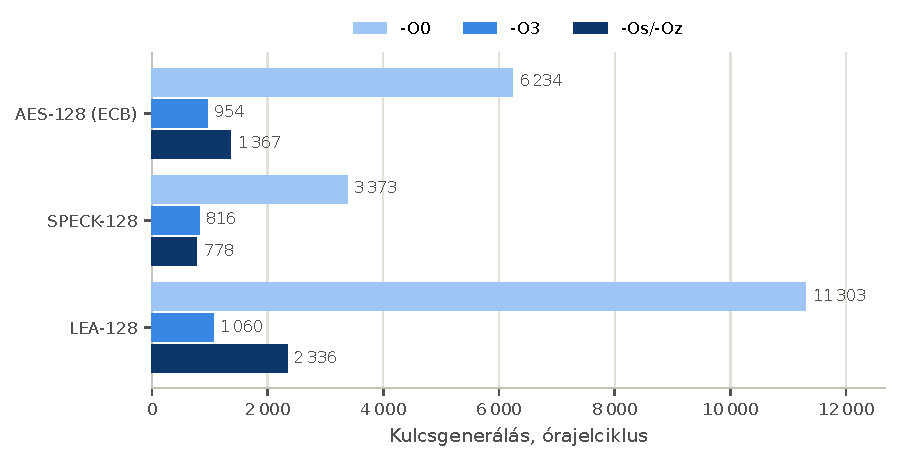
\includegraphics[width=0.8\textwidth]{5_kulcsgeneralas}
    \caption{A kulcsgenerálás ciklusszáma \texttt{-O0}, \texttt{-O3} és \texttt{-Os/-Oz} mellett. Az ASCON-128 nem szerepel, mert nincs külön kulcsgenerálási lépése.}
    \label{fig:keygen}
\end{figure}

Az \texttt{-O0}-ról \texttt{-O3}-ra váltva a kulcsgenerálás az AES-nél 6,5-szer, a SPECK-nél 4,1-szer, a LEA-nál 10,7-szer gyorsult. Optimalizálás nélkül a LEA a legdrágább, mert körönként hat körkulcsszót kell előállítania, és a sok kis segédfüggvény (forgatás, konstansszámítás) mind külön hívás. Sebességre optimalizált kódban (\texttt{-O2}, \texttt{-O3}, \texttt{-Ofast}) a három algoritmus közel azonos, 800--1150 ciklus. Az \texttt{-Os/-Oz} szinten a LEA kulcsgenerálása ismét kétszer drágább, valószínűleg azért, mert a fordító a konstansszámító segédfüggvényt nem ágyazza be (ezt a külön fordításban, \ref{sec:memoria}.~alfejezet, láttuk); a SPECK-é viszont itt a leggyorsabb (778 ciklus).

Az ASCON-128 nem használ külön kulcskiterjesztést: a kulcsot az inicializáláskor és a véglegesítéskor keveri be (\ref{sec:ascon_aead}.~alfejezet), így ez a költség a titkosítás mért idejében jelenik meg. Gyakorlati szempontból a kulcsgenerálás akkor számít, ha a kulcs gyakran változik: \texttt{-O3} mellett a LEA kulcsgenerálása nagyjából egy blokk titkosításának, az AES-é egy blokk ötödének felel meg.

\section{Titkosítás és visszafejtés}\label{sec:aszimmetria}

A~\ref{fig:cpb_o3}.~ábra a fajlagos költséget (ciklus/bájt, cycles per byte, CPB) mutatja 1024 bájtos üzeneten \texttt{-O3} mellett. A többi szint értékei az~\ref{fig:hoterkep}.~ábrán láthatók.

\begin{figure}[htbp]
    \centering
    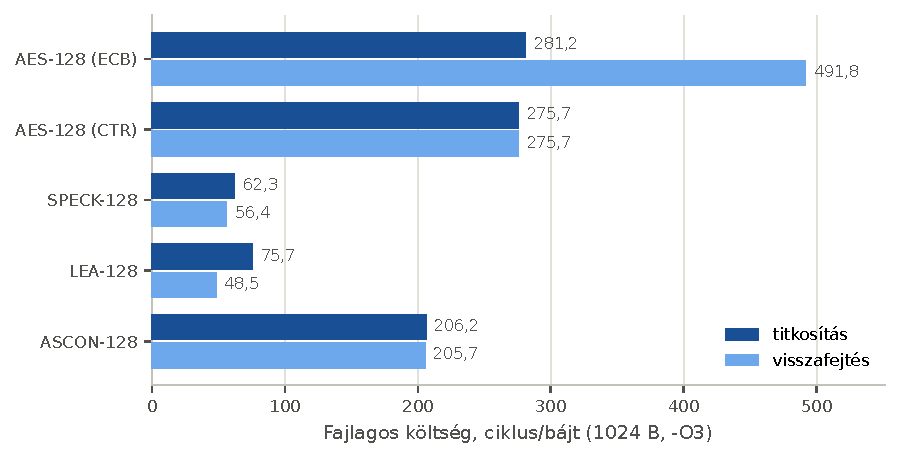
\includegraphics[width=0.8\textwidth]{2_cpb_O3}
    \caption{Fajlagos költség 1024 bájtos üzeneten, \texttt{-O3} mellett}
    \label{fig:cpb_o3}
\end{figure}

Az AES ECB módban erősen aszimmetrikus: a visszafejtés \texttt{-O0} mellett 9,1-szer, \texttt{-O3} mellett 1,75-ször drágább a titkosításnál. Ezt az inverz MixColumns magyarázza, amely a használt implementációban blokkonként negyvenszer annyi \texttt{xtime} hívást tartalmaz, mint a titkosító irány (\ref{sec:megvalositas}.~alfejezet). Optimalizálás nélkül minden ilyen hívás valódi függvényhívás, ezért a különbség óriási. \texttt{-O3} mellett a fordító beágyazza a függvényt, és mivel a szorzó együtthatók konstansok, a felesleges tagok és az ismétlődő számítások nagy részét kiejtheti, így az aszimmetria jóval kisebb lesz. CTR módban a két irány költsége minden szinten azonos (\texttt{-O3} mellett 275,7 CPB), mert a visszafejtés is a titkosító függvényt hívja. Az aszimmetria tehát az inverz blokkművelet költsége, amelyet megfelelő üzemmóddal el lehet kerülni.

Az ASCON-128 két iránya szintén azonos költségű (\texttt{-O3} mellett 206,2 és 205,7 CPB), mert a duplexkonstrukcióban mindkét irány ugyanazt a permutációt futtatja. A SPECK visszafejtése minden szinten kb.\ 10\,\%-kal gyorsabb a titkosításnál. A LEA-nál \texttt{-O0} mellett a két irány gyakorlatilag azonos, \texttt{-O3} mellett viszont a visszafejtés (48,5 CPB) jóval gyorsabb a titkosításnál (75,7 CPB), és ezzel a teljes mérés leggyorsabb művelete. Mivel a különbség csak optimalizált kódban jelentkezik, és szintenként változik (\ref{sec:optimalizacio}.~alfejezet), valószínűleg a fordító által generált kódból ered, nem magából az algoritmusból.

\section{Skálázódás az üzenetmérettel}\label{sec:skalazodas}

A~\ref{fig:skal}.~ábra a titkosítás idejét mutatja az üzenetméret függvényében, az~\ref{tab:cikl_o3}.~táblázat pedig a mért ciklusszámokat, mindkettő \texttt{-O3} mellett.

\begin{figure}[htbp]
    \centering
    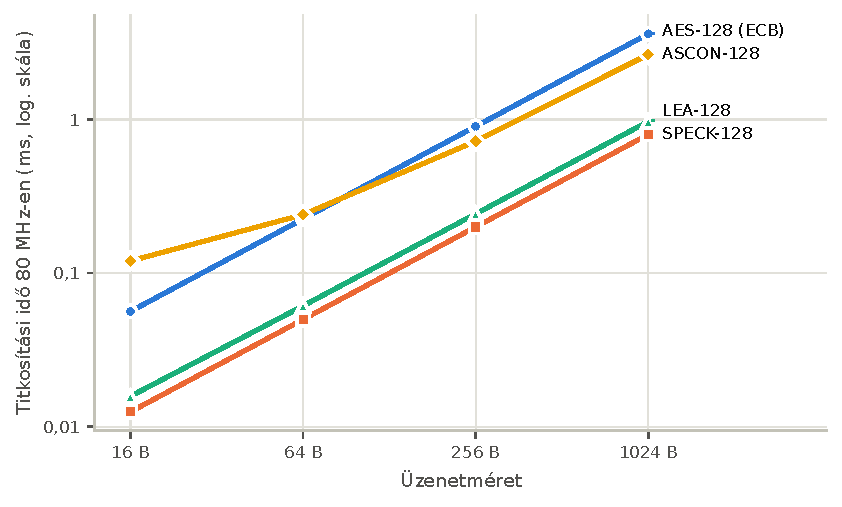
\includegraphics[width=0.8\textwidth]{1_skalazodas}
    \caption{A titkosítás ideje az üzenetméret függvényében (\texttt{-O3}, 80~MHz, mindkét tengely logaritmikus)}
    \label{fig:skal}
\end{figure}

\begin{table}[htbp]
    \centering
    \small
    \caption{A titkosítás ciklusszáma az üzenetméret függvényében (\texttt{-O3})}
    \label{tab:cikl_o3}
    \begin{tabular}{|l|r|r|r|r|}
        \hline
        \textbf{Algoritmus} & \textbf{16 B} & \textbf{64 B} & \textbf{256 B} & \textbf{1024 B} \\ \hline
        AES-128 (ECB) & 4\,500  & 18\,002 & 71\,988 & 287\,937 \\ \hline
        AES-128 (CTR) & 4\,508  & 17\,754 & 70\,752 & 282\,362 \\ \hline
        SPECK-128     & 1\,000  & 3\,991  & 15\,955 & 63\,811  \\ \hline
        LEA-128       & 1\,263  & 4\,893  & 19\,413 & 77\,493  \\ \hline
        ASCON-128     & 9\,592  & 19\,192 & 57\,592 & 211\,192 \\ \hline
    \end{tabular}
\end{table}

A blokktitkosítók költsége egyenesen arányos az üzenet hosszával: ECB módban minden 16 bájtos blokk ugyanannyiba kerül, így a CPB minden méreten gyakorlatilag állandó (az AES-é 16 bájton 281,3, 1024 bájton 281,2). A logaritmikus ábrán ezért párhuzamos egyeneseket látunk.

Az ASCON-128 viselkedése eltér ettől: CPB-je 16 bájton 600, 1024 bájton 206. A négy mérési pont \texttt{-O3} mellett pontosan illeszkedik a
\begin{equation}
	C_{\mathrm{ASCON}}(n) \approx 6\,392 + 200 \cdot n
\end{equation}
egyenesre, ahol $n$ az üzenet hossza bájtban. Mindkét tag visszavezethető a felépítésre. A meredekség azt jelenti, hogy egy 8 bájtos blokk 1600 ciklusba kerül, és mivel minden blokkhoz egy 6 körös permutáció tartozik, egy permutációs kör kb.\ 267 ciklus. A tengelymetszet ennek nagyjából 24-szerese, ami pontosan az inicializálás és a véglegesítés két 12 körös permutációja. Ellenőrzésképpen: 16 bájtnál két adatblokk és a két fix permutáció összesen 36 kört jelent, ami $36 \times 267 \approx 9\,600$ ciklus, a mért érték 9\,592.

Ebből következik, hogy az ASCON-128 rövid üzeneteken lassabb az AES-nél, hosszabbakon gyorsabb (\ref{fig:ascon_aes}.~ábra). Az összevetés nem azonos szolgáltatások között történik: az ASCON a hitelesítő címkét is kiszámítja, az ECB és a CTR módú AES nem. A két egyenes \texttt{-O3} mellett kb.\ 79 bájtnál metszi egymást (CTR módú AES-sel kb.\ 83 bájtnál). Az átfordulási pont erősen függ a fordítási szinttől: \texttt{-O2} mellett kb.\ 54 bájt, \texttt{-Os/-Oz} mellett, ahol az ASCON a leggyorsabb, az AES pedig lassú, már kb.\ 23 bájt. Egy hitelesítést is nyújtó AES-alapú séma ennél drágább lenne: CCM módban például blokkonként két AES-hívás kell (egy a CBC-MAC-hez, egy a CTR-titkosításhoz), így ott az átfordulási pont jóval alacsonyabbra kerülne. Ezt nem mértük.

\begin{figure}[htbp]
    \centering
    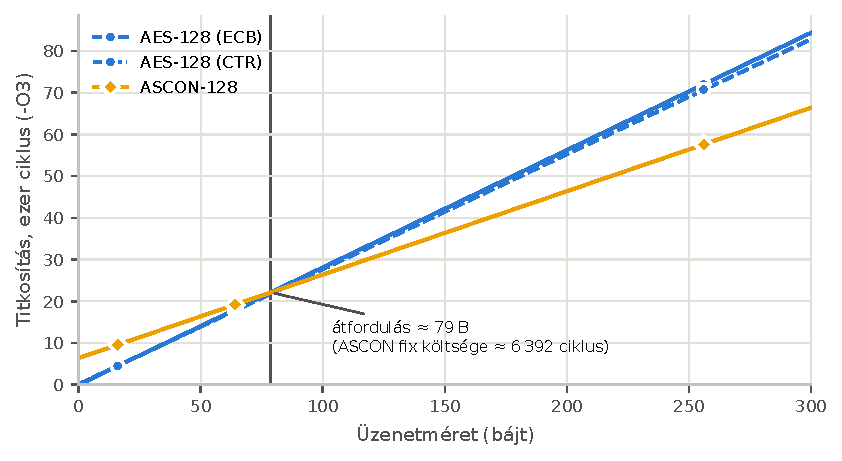
\includegraphics[width=0.8\textwidth]{6_ascon_vs_aes}
    \caption{Az ASCON-128 és az AES-128 titkosítási költsége rövid üzeneteken (\texttt{-O3}); a vonalak a mérési pontokra illesztett egyenesek}
    \label{fig:ascon_aes}
\end{figure}

A szabványos Ascon-AEAD128 költségére ebből becslést is adhatunk. Az ASCON-128a paramétereivel 16 bájtonként 8 kör fut, vagyis bájtonként 0,5 kör a 0,75 helyett. Változatlan körköltséggel számolva a meredekség kb.\ 133 ciklus/bájtra csökkenne, a fix költség nem változna, és az AES-szel való átfordulás \texttt{-O3} mellett kb.\ 43 bájtra kerülne. Ez csak becslés, amelyet méréssel kell ellenőrizni (\ref{sec:tovabbfejlesztes}.~alfejezet).

\section{Feldolgozási sebesség}\label{sec:atvitel}

A feldolgozási sebesség (throughput) azt mutatja, hány bájtot tud a mikrovezérlő másodpercenként titkosítani vagy visszafejteni; ez nem azonos a kommunikációs csatorna átviteli sebességével. Az órajelből és a fajlagos költségből adódik: $v = f_{\mathrm{CLK}}/\mathrm{CPB}$, ahol 1~kB $=$ 1000~B. Az 1024 bájtos üzenetre vonatkozó értékeket az~\ref{tab:throughput}.~táblázat mutatja a gyakorlatban leginkább használt három szinten.

\begin{table}[htbp]
    \centering
    \small
    \caption{Feldolgozási sebesség 1024 bájtos üzeneten, 80~MHz-en (kB/s; T: titkosítás, V: visszafejtés)}
    \label{tab:throughput}
    \begin{tabular}{|l|r|r|r|r|r|r|}
        \hline
        \textbf{Algoritmus} & \multicolumn{2}{c|}{\textbf{\texttt{-O2}}} & \multicolumn{2}{c|}{\textbf{\texttt{-O3}}} & \multicolumn{2}{c|}{\textbf{\texttt{-Os/-Oz}}} \\ \cline{2-7}
        & T & V & T & V & T & V \\ \hline
        AES-128 (ECB) & 220    & 129    & 285    & 163    & 179    & 103    \\ \hline
        AES-128 (CTR) & 214    & 214    & 290    & 290    & 172    & 172    \\ \hline
        SPECK-128     & 1\,284 & 1\,419 & 1\,284 & 1\,419 & 1\,283 & 1\,417 \\ \hline
        LEA-128       & 1\,135 & 1\,581 & 1\,057 & 1\,650 & 1\,387 & 1\,484 \\ \hline
        ASCON-128     & 340    & 334    & 388    & 389    & 412    & 413    \\ \hline
    \end{tabular}
\end{table}

A legnagyobb feldolgozási sebességet a LEA visszafejtése érte el \texttt{-O3} mellett (1\,650~kB/s). Titkosításban a legjobb érték a LEA-é \texttt{-Os/-Oz} mellett (1\,387~kB/s), a SPECK pedig minden optimalizált szinten 1\,284~kB/s-ot ért el. Ugyanazon a szinten (\texttt{-O3}) a leglassabb művelet, az AES ECB-visszafejtése és a leggyorsabb között tízszeres a különbség.

Az ASCON-128 \texttt{-O3} mellett kb.\ 1,3-szer, \texttt{-Os/-Oz} mellett 2,4-szer gyorsabb a CTR módú AES-nél, miközben a hitelesítő címkét is kiszámítja. A csak titkosságot nyújtó SPECK-nél és LEA-nál viszont 2,7--4,2-szer lassabb.

\section{Kódméret és memóriaigény}\label{sec:memoria}

A kódméretet és a veremigényt a mérőprogrammal azonos kapcsolókkal végzett külön fordításból határoztuk meg. A flash-igény a linker térképfájljából (\texttt{.map}) adódik, a nem használt függvényeket eltávolító \texttt{--gc-sections} linkelés után, a veremigény pedig a GCC \texttt{-fstack-usage} és \texttt{-fcallgraph-info} kapcsolójának kimenetéből, a hívási lánc mentén összegezve. Ehhez a fordításhoz az arm-none-eabi-gcc 13.3.1-es verzióját használtuk, ezért a bájtértékek a mérésnél használt 14.3.1-es fordítóétól kis mértékben eltérhetnek, az arányok azonban nem. % TODO: ha a saját (14.3.1-es) build .map és .su fájljaiból is megvannak az értékek, ezekre cserélhetők.
Az eredményeket az~\ref{tab:memoria}.~táblázat foglalja össze.

\begin{table}[htbp]
    \centering
    \small
    \caption{Flash-igény (kód és konstansok) és legnagyobb veremhasználat bájtban, a mért függvényekre}
    \label{tab:memoria}
    \begin{tabular}{|l|r|r|r|r|r|r|r|r|}
        \hline
        \textbf{Algoritmus} & \multicolumn{4}{c|}{\textbf{Flash (B)}} & \multicolumn{4}{c|}{\textbf{Verem (B)}} \\ \cline{2-9}
        & \texttt{-O0} & \texttt{-O2} & \texttt{-O3} & \texttt{-Os} & \texttt{-O0} & \texttt{-O2} & \texttt{-O3} & \texttt{-Os} \\ \hline
        AES-128\textsuperscript{*} & 4\,135 & 1\,995 & 3\,995 & 1\,541 & 120 & 88 & 176 & 108 \\ \hline
        SPECK-128 & 778 & 292 & 292 & 280 & 88 & 32 & 32 & 20 \\ \hline
        LEA-128\textsuperscript{\dag} & 3\,168 & 1\,508 & 1\,508 & 1\,358 & 152 & 88 & 88 & 88 \\ \hline
        ASCON-128 & 3\,202 & 22\,784 & 27\,208 & 1\,768 & 688 & 256 & 232 & 240 \\ \hline
    \end{tabular}
    \begin{flushleft}
    \footnotesize
    Az \texttt{-Ofast} értékei az \texttt{-O3}-éval, az \texttt{-Oz} értékei az \texttt{-Os}-éval azonosak. A veremigény a könyvtári \texttt{memcpy} nélkül értendő.\\
    \textsuperscript{*}Az ECB- és a CTR-módot, valamint a 2\,$\times$\,256 bájtos S-box-táblákat is tartalmazza.\\
    \textsuperscript{\dag}A 192 és 256 bites kulcs kezelését is tartalmazza.
    \end{flushleft}
\end{table}

A kulcsfüggő adatok a RAM-ban külön helyet foglalnak: az AES kontextusa 192 bájt (176 bájt körkulcs és a CTR-mód 16 bájtos számlálója), a SPECK 32 körkulcsa 256 bájt, a LEA kulcsstruktúrája 772 bájt, amelyből 128 bites kulcsnál 576 bájt van használatban. Az ASCON-nak nincs tárolt körkulcsa, a 40 bájtos állapot a veremben van, és a táblázat veremértéke már tartalmazza. A mérőprogram saját puffereit (3\,$\times$\,1040 bájt) nem számoltuk az algoritmusokhoz, mert ezek az alkalmazástól függnek.

A legfeltűnőbb az ASCON: \texttt{-Os} mellett 1,8~KB, \texttt{-O2} és \texttt{-O3} mellett viszont 22--27~KB. Ennek oka, hogy a forrásban a \texttt{ROUND}, a \texttt{P6} és a \texttt{P12} \texttt{static inline} függvény, ezért sebességre optimalizálva a fordító a köröket kibontja, és a 12, illetve 6 körös permutációt minden hívási helyre külön beágyazza. Méretre optimalizálva ezt nem teszi meg. Csak a kapcsolódó adatot feldolgozó segédfüggvény, amely két 6 körös permutációt tartalmaz, 4,5~KB; egyetlen kibontott 6 körös permutáció tehát kb.\ 2~KB, ami jóval nagyobb az ART 1~KB-os utasítás-gyorsítótáránál. \texttt{-Os} mellett a \texttt{ROUND} függvény 394 bájt, és egy ciklus hívja, így a teljes forró kódrész elfér a gyorsítótárban. Ennek a sebességre gyakorolt hatását a következő alfejezet tárgyalja.

A SPECK kódja minden szinten néhány száz bájt, mert egy körfüggvényből áll, amelyet a kulcsgenerálás is használ. 8 és 16 bites eszközökön, ahol a flash néhány tíz kilobájt (\ref{sec:mikrovezerlok}.~alfejezet), a kódméret önmagában is kizárhat egy változatot; az ASCON-t ilyen eszközre méretre optimalizálva érdemes fordítani.

\section{A fordítói optimalizáció hatása}\label{sec:optimalizacio}

Az~\ref{fig:hoterkep}.~ábra minden algoritmus és minden szint fajlagos költségét mutatja, a~\ref{fig:relativ}.~ábra pedig az \texttt{-O3}-hoz viszonyított eltérést.

\begin{figure}[htbp]
    \centering
    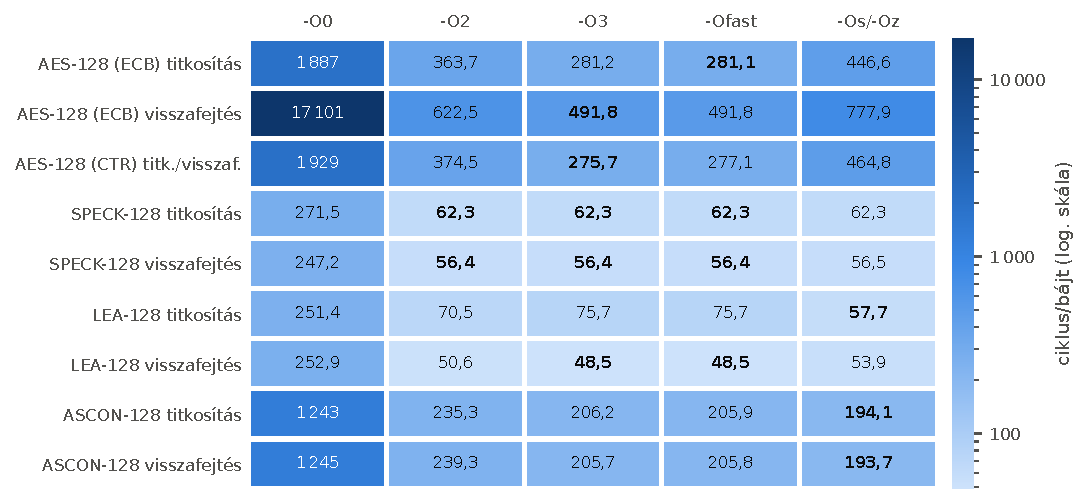
\includegraphics[width=\textwidth]{3_cpb_hoterkep}
    \caption{Fajlagos költség (ciklus/bájt) 1024 bájtos üzeneten, minden optimalizációs szinten. Soronként félkövér a legjobb érték.}
    \label{fig:hoterkep}
\end{figure}

\begin{figure}[htbp]
    \centering
    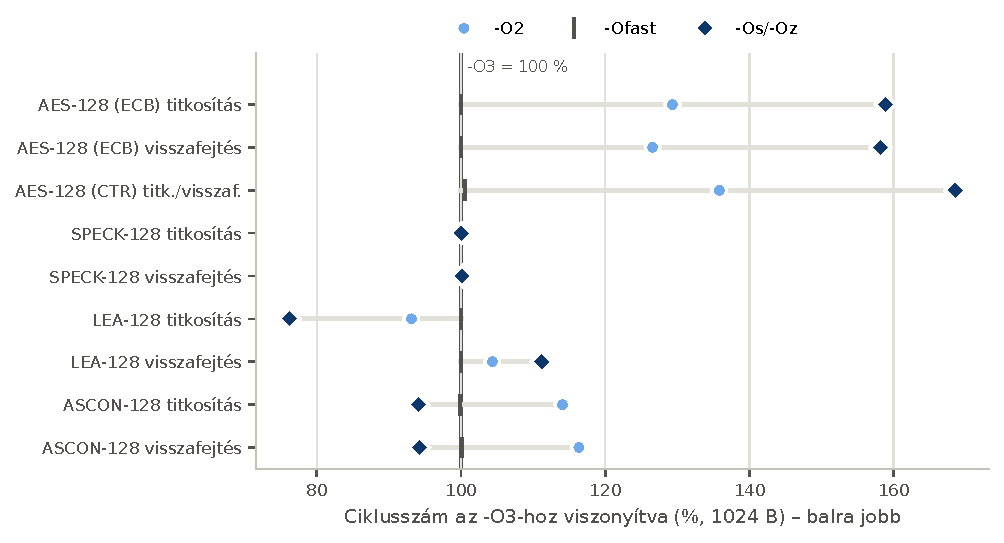
\includegraphics[width=0.85\textwidth]{4_relativ_O3}
    \caption{A ciklusszám az \texttt{-O3}-on mért érték százalékában (1024 B); 100\,\% alatt az adott szint gyorsabb}
    \label{fig:relativ}
\end{figure}

\subsection{Optimalizálás nélkül és optimalizálva}

Az optimalizálás minden algoritmust jelentősen gyorsított: 1024 bájtos titkosításnál \mbox{\texttt{-O0}-hoz} képest \texttt{-O3} mellett az AES 6,7-szer, az ASCON 6,0-szor, a SPECK 4,4-szer, a LEA 3,3-szer gyorsabb. A legnagyobb a különbség az AES ECB-visszafejtésénél: 17,5 millióról 504 ezer ciklusra, azaz 34,8-szeresére gyorsult, ami az előző alfejezetekben leírt \texttt{xtime}-hívásokkal magyarázható. Az \texttt{-O0} eredményei ezért elsősorban azt mutatják, hogy fejlesztői beállítással mért adatokból nem szabad következtetni az algoritmusok valódi költségére.

\subsection{\texttt{-O2}, \texttt{-O3} és \texttt{-Ofast}}

A SPECK már \texttt{-O2} mellett eléri a legjobb értékét, az \texttt{-O3} és az \texttt{-Ofast} sem javít rajta; a rövid, egyszerű körfüggvényen láthatóan nincs mit tovább optimalizálni. Az AES és az ASCON \texttt{-O3} mellett 12--26\,\%-kal kevesebb ciklust igényel, mint \texttt{-O2} mellett, a LEA titkosítása viszont \texttt{-O2} mellett 7\,\%-kal gyorsabb. Az \texttt{-Ofast} a titkosítás és a visszafejtés értékeiben sehol nem tért el 0,5\,\%-nál jobban az \texttt{-O3}-tól; a legnagyobb eltérés az AES kulcsgenerálásánál adódott (954, illetve 972 ciklus, 1,9\,\%), ami valószínűleg a kód elhelyezkedéséből ered. Ez várható volt, mert az \texttt{-Ofast} többlete a lebegőpontos számításokat érinti, a vizsgált algoritmusok pedig csak egész műveleteket használnak.

\subsection{\texttt{-Os/-Oz}}

A méretre optimalizált kód hatása algoritmusonként eltér. Az AES ECB módban kb.\ 58\,\%-kal, CTR módban 69\,\%-kal lassabb, mint \texttt{-O3} mellett, mert a fordító a sok kis segédfüggvényt (\texttt{xtime}, \texttt{AddRoundKey}) nem ágyazza be. A SPECK gyakorlatilag érzéketlen a beállításra (0,2\,\% alatti eltérés). A LEA titkosítása 23,8\,\%-kal gyorsabb, visszafejtése 11,2\,\%-kal lassabb. Az ASCON mindkét irányban kb.\ 6\,\%-kal gyorsabb, mint \texttt{-O3} mellett, és 18\,\%-kal, mint \texttt{-O2} mellett; ezen a szinten éri el a legjobb eredményét.

Az ASCON viselkedésére a kódméret ad magyarázatot (\ref{sec:memoria}.~alfejezet). \texttt{-O2} és \texttt{-O3} mellett a kibontott permutáció nem fér el az ART 1~KB-os utasítás-gyorsítótárában, ezért minden körben újra a flash-ből kell olvasni, 4 várakozási ciklussal, előolvasás nélkül. A kevesebb utasításból álló, de gyorsítótárba férő \texttt{-Os} kód ezt elkerüli. Ezzel összhangban a két nagy kódot adó szint (\texttt{-O2} és \texttt{-O3}) egyaránt lassabb az \texttt{-Os}-nél, pedig több optimalizálást végez. Teljes bizonyításhoz a mérést kikapcsolt utasítás-gyorsítótárral is meg kellene ismételni.

A LEA-nál ez a magyarázat nem elégséges: a kód mindhárom optimalizált szinten 1,3--1,5~KB, és a forró ciklus mindegyiknél elfér a gyorsítótárban. Itt valószínűleg a generált utasítássorrend és a regiszterkiosztás különbsége okozza az eltérést, amit a generált assembly összevetésével lehetne igazolni. A gyakorlati következmény mindenesetre az, hogy \texttt{-Os/-Oz} mellett a LEA titkosítása gyorsabb a SPECK-nél (57,7, illetve 62,3 CPB), \texttt{-O3} mellett pedig fordítva.

\subsection{A mérések ismételhetősége}

A SPECK és a LEA \texttt{-O3} értékei ciklusra megegyeztek a mérőprogram korábbi, más szerkezetű változatával végzett mérésekkel, az \texttt{-Os} és az \texttt{-Oz} pedig azonos kód mellett azonos eredményt adott. Ezek, valamint a körök közötti 0,022\,\% alatti eltérés azt mutatják, hogy a mérés stabil, és a fenti különbségek a kódból, nem a mérési zajból származnak. Ez a kontrollált benchmarkra érvényes, nem valós üzemi terhelésre.

\section{Az eredmények összegzése}\label{sec:osszesites}

\texttt{-O3} mellett 1024 bájtos üzeneten az ARX-alapú SPECK és LEA fajlagos költsége titkosításkor 3,7--4,5-ször, visszafejtéskor 8,7--10-szer kisebb, mint a vizsgált \texttt{tiny-AES-c} implementációé ECB módban. Az ASCON-128 a beépített hitelesítés ellenére kb.\ 80 bájt fölött gyorsabb a hitelesítést nem végző ECB és CTR módú AES-nél, rövid üzeneteknél viszont a két 12 körös permutáció kb.\ 6\,400 ciklusos fix költsége a hátrányára szól. A legjobb fordítási szint algoritmusfüggő: az AES-nek az \texttt{-O3}, az ASCON-nak és a LEA titkosításának az \texttt{-Os/-Oz} kedvez, a SPECK-et alig befolyásolja. Egy adott alkalmazásban ezért nemcsak az algoritmust, hanem a fordítási beállítást is mérés alapján érdemes megválasztani.

% ============================================================
% 6. FEJEZET – BIZTONSÁGI ELEMZÉS
% ============================================================
\chapter{Biztonsági elemzés és összehasonlító értékelés}\label{chap:biztonsag}

A teljesítmény mellett legalább ilyen fontos, hogy egy algoritmus milyen védelmet nyújt az ismert támadásokkal szemben. Ez a fejezet a szakirodalom alapján foglalja össze a négy algoritmus biztonsági jellemzőit; támadásokat nem valósítottunk meg.

% -------------------------------------------------------
\section{Alapfogalmak}\label{sec:kriptoanalizis_alap}
% -------------------------------------------------------

\subsection{Támadási modellek}

A támadó képességei szerint négy, egyre erősebb modellt szokás megkülönböztetni \cite{Stallings2017}. A \emph{csak titkosított szöveget ismerő} (ciphertext-only) támadó kizárólag a titkosított kimenetet látja. Az \emph{ismert nyílt szöveges} (known-plaintext) modellben nyílt és titkosított szövegpárok is rendelkezésére állnak. A \emph{választott nyílt szöveges} (chosen-plaintext, CPA) modellben maga választhatja meg a titkosítandó üzeneteket; ez reálisabb, mint elsőre tűnik, mert sok protokollban a támadó rá tudja venni az eszközt bizonyos üzenetek titkosítására. A \emph{választott titkosított szöveges} (chosen-ciphertext, CCA) modellben a visszafejtendő szövegeket is ő választja. A modern algoritmusoktól általában a CPA- vagy a CCA-modellben várnak el biztonságot.

\subsection{Biztonsági szint és biztonsági tartalék}

Egy algoritmus \emph{biztonsági szintje} $s$ bit, ha a legjobb ismert támadás $2^s$ műveletet igényel. Ideális esetben ez a kulcs hossza, vagyis a legjobb támadás a kulcstér végigpróbálása, ami 128 bites kulcsnál $2^{128} \approx 3{,}4 \times 10^{38}$ művelet.

A \emph{biztonsági tartalék} (security margin) azt fejezi ki, hogy az algoritmus teljes körszáma ($N$) mennyivel több a legjobb ismert támadás által elért körszámnál ($n$): $N - n$ kör, vagy arányosan $(N-n)/N$. Minél nagyobb a tartalék, annál több tér marad a jövőbeli, erősebb támadások számára \cite{Biryukov2017}. Eltérő körszámú algoritmusokat csak az arányos értékkel lehet összevetni.

% -------------------------------------------------------
\section{A főbb támadástípusok}\label{sec:tamadastipusok}
% -------------------------------------------------------

\subsection{Differenciális kriptoanalízis}

A differenciális kriptoanalízist Biham és Shamir vezette be 1991-ben a DES elemzésére \cite{Biham1991}. A támadó olyan nyíltszöveg-párokat választ, amelyek között ismert (általában XOR-) különbség van, és azt vizsgálja, hogyan terjed ez a különbség a körökön át. Ha bizonyos bemeneti különbségek a véletlennél nagyobb valószínűséggel adnak bizonyos kimeneti különbségeket, abból a körkulcsok egyes bitjeire lehet következtetni. A tervezők ezért úgy választják meg az S-boxokat és a körszámot, hogy a teljes titkosításon átívelő differenciális jellemzők valószínűsége elhanyagolható legyen. ARX-algoritmusoknál az elemzés nehezebb, mert a moduláris összeadás differenciális viselkedése az átvitelek miatt bonyolultabb, mint egy S-boxé.

\subsection{Lineáris kriptoanalízis}

Matsui 1993-ban publikálta a lineáris kriptoanalízist, szintén a DES-re \cite{Matsui1993}. A támadó a nyílt szöveg, a titkosított szöveg és a kulcs bitjei közötti olyan lineáris (XOR-) összefüggéseket keres, amelyek a véletlennél gyakrabban teljesülnek; elég sok ismert szövegpárból ezekkel kulcsbitek nyerhetők ki. Bogdanov és Rijmen később bevezették a nulla korrelációjú lineáris kriptoanalízist \cite{Bogdanov2014}, a differenciális és a lineáris módszer kombinációja, a differenciális-lineáris támadás pedig az ARX-algoritmusok ellen az egyik leghatékonyabbnak bizonyult \cite{Chen2023}.

\subsection{Algebrai és rotációs támadások}

Az algebrai támadások az algoritmust $GF(2)$ feletti egyenletrendszerként írják fel, és ennek megoldásával próbálják meghatározni a kulcsot. A teljes körszámú algoritmusok egyenletrendszere azonban túl nagy a mai megoldók (Gröbner-bázisok, SAT-megoldók) számára, az ARX-algoritmusoknál pedig a moduláris összeadás bitszintű leírása még bonyolultabb egyenletekhez vezet \cite{Biryukov2017}.

A Khovratovich és Nikolić által bevezetett rotációs kriptoanalízis \cite{Khovratovich2010} kifejezetten ARX-szerkezetek ellen készült. Azt használja ki, hogy elforgatott bemenetre egy ideális ARX-rendszer kimenete is elforgatva jelenne meg; ezt az összefüggést a moduláris összeadás és a körkonstansok megtörik, a támadás pedig azt vizsgálja, mennyire. A SPECK és a LEA teljes változata ellen ez a módszer sem vezetett eredményre.

\subsection{Oldalcsatorna-támadások}

Az oldalcsatorna-támadások nem az algoritmus matematikai szerkezetét, hanem a fizikai megvalósítást használják ki \cite{Kocher1996}: a végrehajtási idő, az áramfelvétel (egyszerű és differenciális teljesítményanalízis, SPA és DPA), az elektromágneses kisugárzás vagy a gyorsítótár-hozzáférések mintázata információt hordozhat a kulcsról.

Az \emph{időzítéses} és \emph{gyorsítótár-alapú} támadások ellen a konstans idejű kód véd. A táblás AES-megvalósításokban az S-box-olvasás címe a kulcstól függ, így gyorsítótárral rendelkező rendszereken a hozzáférési idő elvben árulkodó lehet. Az ARX-algoritmusok és az ASCON bitsliced S-boxa nem használ adatfüggő memóriacímet vagy elágazást, ezért természetüknél fogva konstans idejű. A \emph{teljesítményanalízis} ellen viszont a konstans idejűség nem véd: ehhez maszkolás (a köztes értékek véletlen részekre bontása) szükséges. A maszkolás az alacsony fokú S-boxot használó ASCON-nál viszonylag olcsó, ez a tervezők kifejezett célja volt \cite{Dobraunig2021}; az ARX-algoritmusoknál a moduláris összeadás, az AES-nél a nagy S-box miatt drágább.

Oldalcsatorna-méréseket nem végeztünk, mert ehhez oszcilloszkóp és speciális mérőeszközök szükségesek; ez a szakasz a szakirodalmi áttekintés része.

\subsection{Születésnapi korlát}\label{sec:birthday}

A születésnapi paradoxon miatt $n$ bites blokkméret mellett nagyjából $2^{n/2}$ blokk feldolgozása után nagy valószínűséggel ismétlődik egy titkosított blokk. CBC módban például két titkosított blokk egyezéséből a megfelelő nyíltszöveg-blokkok XOR-ja kiszámítható, és a CBC-MAC is hamisíthatóvá válik. A vizsgált blokktitkosítók 128 bites blokkmérete mellett ez a korlát $2^{64}$ blokk, ami IoT-alkalmazásokban gyakorlatilag elérhetetlen. Ezért vizsgáltuk a 64 bites blokkméretű változatok helyett a 128 biteseket.

% -------------------------------------------------------
\section{Az algoritmusok biztonsági jellemzői}\label{sec:alg_security}
% -------------------------------------------------------

\subsection{AES-128}

Az AES-128 a legalaposabban vizsgált blokktitkosítók egyike. A legjobb ismert kulcsvisszafejtő támadások, például a meet-in-the-middle támadások, a 10 körből 7-et érnek el \cite{Derbez2013}, ami 3 kör, azaz 30\,\% tartalék. A teljes algoritmus ellen a legjobb ismert eljárás a biclique-támadás, amely a kulcstér végigpróbálásához képest mindössze kb.\ négyszeres gyorsulást ér el ($2^{126{,}1}$ művelet), így gyakorlati jelentősége nincs \cite{Bogdanov2011}.

\subsection{SPECK~128/128}

A SPECK~128/128 ellen a legjobb publikált támadás differenciális, és a 32 körből 23-at ér el, közel a kulcstér végigpróbálásának költségével \cite{Song2016}. Ez 9 kör, azaz kb.\ 28\,\% tartalék; a tervezők a körszámot kifejezetten úgy választották meg, hogy a tartalék az AES-éhez hasonló legyen \cite{Beaulieu2017}. Rotációs támadás a teljes változat ellen nem ismert.

\subsection{LEA-128}

A LEA-128 ellen a legjobb ismert támadás differenciális-lineáris, és a 24 körből 17-et ér el \cite{Chen2023}. Ez 7 kör, azaz kb.\ 29\,\% tartalék. A tervezők részletes biztonsági elemzést közöltek a forgatási paraméterek megválasztásáról és a differenciális, illetve lineáris tulajdonságokról \cite{Hong2013}, az algoritmus pedig ISO/IEC-szabvány része \cite{ISO29192}.

\subsection{ASCON-128}

Az ASCON biztonságát AEAD-sémaként kell értékelni. A tervezők a titkosságra és a hitelességre egyaránt 128 bites biztonságot állítanak. A leghosszabb ismert kulcsvisszafejtő támadások a 12 körös inicializálásból 7 kört érnek el, ami 5 kör, azaz kb.\ 42\,\% tartalék \cite{Dobraunig2021,Rohit2021}. A nonce-ismétlést nem igénylő legjobb ilyen támadás kb.\ $2^{123}$ műveletet és $2^{64}$ adatot igényel \cite{Rohit2021}. A két változat inicializálása szerkezetében azonos (csak a kezdőérték különbözik), ezért ez az eredmény várhatóan a 128a-ra is átvihető. Az ASCON-128 256 bites capacity-je ráadásul nagyobb tartalékot hagy, mint a 128a 192 bites capacity-je. Megvalósítási szempontból előnyös, hogy konstans idejű, és viszonylag olcsón maszkolható.

Mint minden nonce-alapú AEAD-sémánál, az ASCON-nál is kritikus, hogy ugyanazzal a kulccsal egy nonce ne ismétlődjön: azonos kulcs, nonce és kapcsolódó adat mellett a két titkosítás ugyanabból az állapotból indul, ezért az első blokkok (és az azonos előtag utáni első eltérő blokk) nyílt szövegeinek XOR-ja kiolvasható a titkosított szövegekből. Az első eltérő blokk után az állapotok szétválnak, a további blokkokra ez már nem érvényes, a titkossági és hitelességi garanciák viszont így is elvesznek. Ez a séma használati feltétele, amelyet az alkalmazásban (például számlálóalapú nonce-szal) kell biztosítani; a mérésekben használt csupa nulla nonce csak mérési célt szolgált.

% -------------------------------------------------------
\section{Összehasonlító értékelés}\label{sec:security_compare}
% -------------------------------------------------------

A~\ref{table:security_compare}.~táblázat a fenti jellemzőket foglalja össze.

\begin{table}[h!]
\centering
\caption{A vizsgált algoritmusok biztonsági jellemzői a szakirodalom alapján}
\label{table:security_compare}
\footnotesize
\vspace{.2 cm}
\setlength{\tabcolsep}{3.5pt}
\begin{tabular}{lcccc}
\hline
\textbf{Szempont} & \textbf{AES-128} & \textbf{SPECK 128/128} & \textbf{LEA-128} & \textbf{ASCON-128} \\
\hline
Állított biztonság & 128 bit & 128 bit & 128 bit & 128 bit \\
Legjobb támadás (kör) & 7 / 10 & 23 / 32 & 17 / 24 & 7 / 12\textsuperscript{a} \\
Támadás típusa & MITM & differenciális & diff.-lineáris & cube-típusú\textsuperscript{a} \\
Biztonsági tartalék & 30\,\% & 28\,\% & 29\,\% & 42\,\% \\
Konstans idejű kód & nehéz\textsuperscript{b} & természetes & természetes & természetes \\
Maszkolás költsége & nagy & nagy & nagy & kisebb \\
Szabvány & FIPS 197 & ISO/IEC 29167-22\textsuperscript{d} & ISO/IEC 29192-2 & SP 800-232\textsuperscript{c} \\
\hline
\end{tabular}
\begin{flushleft}
\footnotesize
\textsuperscript{a}Az inicializáló permutáció 12 köréből.\\
\textsuperscript{b}Táblás megvalósításban; bitsliced szoftveres vagy hardveres megvalósítással megoldható.\\
\textsuperscript{c}A szabványos Ascon-AEAD128 az ASCON-128a változatból készült.\\
\textsuperscript{d}Csak RFID-légi interfészhez.\\
A támadások modellje, adat- és időigénye eltér, ezért a tartalékok csak tájékoztató jellegűek.
\end{flushleft}
\end{table}

A három blokktitkosító arányos biztonsági tartaléka hasonló (28--30\,\%), az ASCON inicializálásáé ennél nagyobb. Ebből csak annyi következik, hogy a publikált támadások egyik blokktitkosító teljes körszámához sem jutottak lényegesen közelebb, mint a többiéhez. Azonos biztonsági szintet ez nem bizonyít. A támadások modellje, adat- és időigénye eltér: a SPECK 23 körös támadása például kb.\ $2^{125}$ választott nyílt szöveget igényel \cite{Song2016}, az AES 7 körös támadásai viszont $2^{100}$ alatti adattal és idővel dolgoznak \cite{Derbez2013}. Az AES-t ráadásul jóval régebben és többen elemzik, mint a két ARX-algoritmust. A gyakorlati különbségek inkább a megvalósításban jelentkeznek. Az ARX-algoritmusok és az ASCON konstans idejű kódja egyszerűbb, mint a táblás AES-é, a teljesítményanalízis elleni maszkolás pedig az ASCON-nál a legolcsóbb. A SPECK hátránya nem kriptoanalitikai, hanem elfogadottsági: az általános célú könnyűsúlyú blokktitkosító-szabványba nem került be, és tervezésének körülményei vitatottak.

% ============================================================
% 7. FEJEZET – ÖSSZEFOGLALÁS
% ============================================================
\chapter{Összefoglalás és továbbfejlesztési lehetőségek}\label{chap:osszefoglalas}

\section{A célkitűzések teljesülése}

A dolgozat célja négy, eltérő felépítésű kriptográfiai algoritmus -- az AES-128, a SPECK~128/128, a LEA-128 és az ASCON-128 -- futásidejű költségének összevetése volt egy valós, ARM Cortex-M4 magos mikrovezérlőn (STM32L432KC). Az algoritmusokat egységes szerkezetű, hivatalos tesztvektorokkal ellenőrzött C-implementációkban valósítottuk meg, és közös, DWT-alapú, ciklusra pontos mérőprogramot írtunk hozzájuk. A kulcsgenerálás, a titkosítás és a visszafejtés költségét négy üzenetméreten és hat optimalizációs szinten, szintenként tíz ismétléssel mértük. Meghatároztuk a kódméretet és a veremigényt is, az eredményeket pedig a szakirodalmi biztonsági elemzéssel együtt értékeltük.

\section{Fő megállapítások}

\textbf{Az ARX-alapú algoritmusok fajlagos költsége lényegesen kisebb.} \texttt{-O3} mellett a SPECK 56--62, a LEA 49--76 ciklust igényelt bájtonként, a vizsgált AES-implementáció 276--492-t; ez titkosításkor 3,7--4,5-szörös, visszafejtéskor 8,7--10-szeres különbség. A SPECK kódja ráadásul optimalizált szinteken 300 bájt alatti.

\textbf{Az AES ECB-visszafejtése jelentős többletköltséggel jár.} 1024 bájton optimalizálás nélkül a visszafejtés 9,1-szer, \texttt{-O3} mellett 1,75-ször drágább a titkosításnál. Az ok az implementáció inverz MixColumns lépése; CTR módban a két irány költsége azonos, így a többlet megfelelő üzemmóddal elkerülhető.

\textbf{Az ASCON-128 hitelesítéssel együtt is versenyképes.} Költsége jó közelítéssel egy kb.\ 6\,400 ciklusos fix tag (a két 12 körös permutáció) és bájtonként kb.\ 200 ciklus összege. Ennek megfelelően \texttt{-O3} mellett kb.\ 80 bájt, \texttt{-Os/-Oz} mellett már kb.\ 23 bájt fölött gyorsabb a hitelesítést nem végző AES-nél, és nincs szüksége külön kulcsgenerálásra.

\textbf{A fordítási beállítás hatása nagy és algoritmusfüggő.} Az optimalizálás az AES-visszafejtést 34,8-szeresére gyorsította, az \texttt{-Ofast} a titkosítás és a visszafejtés értékeiben sehol nem hozott 0,5\,\%-nál nagyobb változást. Az \texttt{-Os} és az \texttt{-Oz} azonos kódot adott. Méretre optimalizálva az ASCON 6\,\%-kal, a LEA titkosítása 24\,\%-kal gyorsabb, az AES 58\,\%-kal lassabb lett, a SPECK-re alig hatott. Az ASCON-nál ezt valószínűleg a kibontott permutáció mérete magyarázza, amely nem fér el az ART-gyorsító 1~KB-os utasítás-gyorsítótárában; ezt a hipotézist kikapcsolt gyorsítótárral végzett méréssel még igazolni kell.

\textbf{A publikált támadások nem jeleznek gyengeséget.} A szakirodalom alapján a három blokktitkosító arányos biztonsági tartaléka hasonló (28--30\,\%), és egyik ellen sem ismert gyakorlatban kivitelezhető támadás. Ez nem jelent bizonyítottan azonos biztonsági szintet, mert a támadások feltételei eltérnek, de nem utal arra, hogy a könnyűsúlyú blokktitkosítók teljesítményelőnye a biztonság rovására menne.

\section{Alkalmazási ajánlások}

A~\ref{tab:ajanlasok}.~táblázat a mérések és a biztonsági elemzés alapján tipikus helyzetekre fogalmaz meg ajánlásokat. Az ajánlások 32 bites Cortex-M4 platformon mért adatokon alapulnak, más architektúrákra csak óvatosan vihetők át.

\begin{table}[htbp]
    \centering
    \small
    \caption{Alkalmazási ajánlások 32 bites mikrovezérlőkre}
    \label{tab:ajanlasok}
    \begin{tabularx}{\textwidth}{|p{4.2cm}|p{3.0cm}|X|}
        \hline
        \textbf{Helyzet} & \textbf{Ajánlás} & \textbf{Indoklás} \\ \hline
        Titkosság és hitelesség is szükséges & ASCON (új fejlesztésnél a szabványos Ascon-AEAD128) & Egy sémában adja a titkosítást és a hitelesítést; a mért ASCON-128 kb.\ 80 bájt fölött (\texttt{-Os} mellett már kb.\ 23 bájt fölött) a hitelesítés nélküli szoftveres AES-nél is gyorsabb. Érdemes méretre optimalizálva fordítani. A szabványos változatot nem mértük. \\ \hline
        Nagy feldolgozási sebesség, a hitelesítést más réteg biztosítja & LEA-128 vagy SPECK~128/128 & A legnagyobb feldolgozási sebesség (1\,000--1\,650~kB/s); a LEA szabványos, a SPECK kódja a legkisebb, és kevésbé érzékeny a fordítási beállításra. \\ \hline
        Nagyon rövid üzenetek, gyakori kulcscsere & SPECK~128/128 vagy LEA-128 & Nincs üzenetenkénti fix költség, és a kulcsgenerálás is olcsó (kb.\ 800--1100 ciklus). \\ \hline
        Szabványmegfelelés (pl.\ FIPS) kötelező vagy van hardveres AES-gyorsító & AES-128 & Hardveres gyorsítóval a szoftveres hátrány megszűnik; szoftveresen CTR-re épülő módban (pl.\ GCM, CCM) érdemes használni, mert az inverz blokkművelet drága. \\ \hline
    \end{tabularx}
\end{table}

A SPECK és a LEA önmagában csak titkosságot nyújt; ha hitelesség is kell, külön MAC-ra vagy hitelesített üzemmódra van szükség, ami a költségüket növeli.

\section{Korlátok}

\begin{itemize}
	\item A mérések egyetlen platformon (STM32L432KC, Cortex-M4) készültek; más architektúrákon, különösen 8 és 16 bites eszközökön, az arányok eltérhetnek.
	\item Az AES-eredmények a méretre optimalizált \texttt{tiny-AES-c} implementációra érvényesek, az ASCON-nál pedig a referenciakódon alapuló megvalósítást mértük; optimalizált (például bitsliced vagy bit-interleaved, assembly) változatokkal a különbségek kisebbek lehetnek.
	\item A blokktitkosítókat ECB módban, az ASCON-t AEAD-ként mértük, így az utóbbi költsége a hitelesítést is tartalmazza; hitelesített AES-módot (GCM, CCM) nem mértünk.
	\item Csak blokkhatárra eső üzenetméreteket (16, 64, 256, 1024 bájt) mértünk, a részleges blokkok kezelésének költségét nem.
	\item Az ASCON-128-at mértük, nem a NIST SP~800-232 szerinti Ascon-AEAD128-at; erre csak becslést adtunk.
	\item A kódméretet a mérésnél használttól eltérő fordítóverzióval határoztuk meg.
	\item Az ART-gyorsítóra vonatkozó magyarázatot kikapcsolt gyorsítótárral végzett méréssel nem ellenőriztük.
	\item Energiafogyasztást és oldalcsatorna-szivárgást nem mértünk; a biztonsági értékelés szakirodalmi adatokon alapul.
\end{itemize}

\section{Továbbfejlesztési lehetőségek}\label{sec:tovabbfejlesztes}

\textbf{A szabványos Ascon-AEAD128 mérése.} A NIST SP~800-232 szerinti változat megvalósítása és mérése megmutatná, mennyire pontos az~\ref{sec:skalazodas}.~alfejezetben adott becslés, és a szabványos sémát a többi algoritmussal közvetlenül is összevethetővé tenné.

\textbf{A gyorsítótár hatásának igazolása.} Az ART utasítás-gyorsítótárának kikapcsolásával, illetve az előolvasás bekapcsolásával végzett mérések eldönthetnék, hogy az ASCON \texttt{-Os/-Oz} melletti előnyét valóban a kódméret okozza-e. A LEA irányfüggő viselkedésének okát a generált assembly összevetése tárhatja fel.

\textbf{Optimalizált implementációk.} Cortex-M-re optimalizált AES- és ASCON-megvalósítások mérése megmutatná, mennyi a különbség az algoritmusok és mennyi a megvalósítási stílus között.

\textbf{További platformok.} A mérések kiterjesztése más Cortex-M magokra (M0+, M33), valamint RISC-V és AVR mikrovezérlőkre megmutatná, mennyire általánosíthatók az eredmények.

\textbf{Energia- és oldalcsatorna-mérés.} Precíziós árammérővel az algoritmusok tényleges energiaigénye, oszcilloszkóppal pedig a teljesítményanalízissel szembeni ellenállásuk is vizsgálható lenne.

\textbf{Azonos funkcionalitású összevetés.} Az AES és a LEA hitelesített üzemmódjainak (például GCM, CCM) mérése lehetővé tenné, hogy az ASCON-t azonos szolgáltatást nyújtó megoldásokkal hasonlítsuk össze.

% ============================================================
% IRODALOMJEGYZÉK
% ============================================================
\newpage
\begin{bibdiv}
\begin{biblist}
 \addcontentsline{toc}{chapter}{Irodalomjegyzék}

\bib{Stallings2017}{book}{
author={W. Stallings},
title={Cryptography and Network Security: Principles and Practice},
edition={7},
publisher={Pearson},
date={2017},
}

\bib{Paar2010}{book}{
author={C. Paar},
author={J. Pelzl},
title={Understanding Cryptography: A Textbook for Students and Practitioners},
publisher={Springer},
date={2010},
}

\bib{Shannon1949}{article}{
author={C. E. Shannon},
title={Communication Theory of Secrecy Systems},
journal={Bell System Technical Journal},
volume={28},
number={4},
date={1949},
pages={656--715},
}

\bib{FIPS197}{book}{
author={NIST},
title={Advanced Encryption Standard (AES), FIPS PUB 197},
publisher={National Institute of Standards and Technology},
date={2001},
}

\bib{DaemenRijmen2002}{book}{
author={J. Daemen},
author={V. Rijmen},
title={The Design of Rijndael: AES -- The Advanced Encryption Standard},
publisher={Springer},
date={2002},
}

\bib{NISTIR8114}{article}{
author={K. A. McKay},
author={L. Bassham},
author={M. S. Turan},
author={N. Mouha},
title={Report on Lightweight Cryptography},
journal={NIST Internal Report 8114},
date={2017},
}

\bib{Biryukov2017}{article}{
author={A. Biryukov},
author={L. Perrin},
title={State of the Art in Lightweight Symmetric Cryptography},
journal={IACR ePrint Archive 2017/511},
date={2017},
}

\bib{Hatzivasilis2018}{article}{
author={G. Hatzivasilis},
author={K. Fysarakis},
author={I. Papaefstathiou},
author={C. Manifavas},
title={A Review of Lightweight Block Ciphers},
journal={Journal of Cryptographic Engineering},
volume={8},
number={2},
date={2018},
pages={141--184},
}

\bib{Dobraunig2021}{article}{
author={C. Dobraunig},
author={M. Eichlseder},
author={F. Mendel},
author={M. Schl\"affer},
title={Ascon v1.2: Lightweight Authenticated Encryption and Hashing},
journal={Journal of Cryptology},
volume={34},
number={3},
date={2021},
}

\bib{NISTLWC2023}{book}{
author={NIST},
title={Lightweight Cryptography Standardization Process: NIST Selects Ascon},
publisher={National Institute of Standards and Technology},
date={2023},
}

\bib{NISTSP800232}{book}{
author={NIST},
title={Ascon-Based Lightweight Cryptography Standards for Constrained Devices (NIST SP 800-232)},
publisher={National Institute of Standards and Technology},
date={2025},
note={Available: https://csrc.nist.gov/pubs/sp/800/232/final},
}

\bib{Beaulieu2013}{article}{
author={R. Beaulieu},
author={D. Shors},
author={J. Smith},
author={S. Treatman-Clark},
author={B. Weeks},
author={L. Wingers},
title={The SIMON and SPECK Families of Lightweight Block Ciphers},
journal={IACR ePrint Archive 2013/404},
date={2013},
}

\bib{Beaulieu2017}{article}{
author={R. Beaulieu},
author={D. Shors},
author={J. Smith},
author={S. Treatman-Clark},
author={B. Weeks},
author={L. Wingers},
title={Notes on the Design and Analysis of SIMON and SPECK},
journal={IACR ePrint Archive 2017/560},
date={2017},
}

\bib{Beaulieu2019}{book}{
author={R. Beaulieu},
author={D. Shors},
author={J. Smith},
author={S. Treatman-Clark},
author={B. Weeks},
author={L. Wingers},
title={SIMON and SPECK Implementation Guide, Version 1.1},
publisher={National Security Agency},
date={2019},
}

\bib{Hong2013}{article}{
author={D. Hong},
author={J.-K. Lee},
author={D.-C. Kim},
author={D. Kwon},
author={K. H. Ryu},
author={D.-G. Lee},
title={LEA: A 128-Bit Block Cipher for Fast Encryption on Common Processors},
journal={WISA 2013, Lecture Notes in Computer Science},
volume={8267},
date={2013},
pages={3--27},
}

\bib{ISO29192}{book}{
author={ISO/IEC},
title={Information security -- Lightweight cryptography -- Part 2: Block ciphers (ISO/IEC 29192-2:2019)},
publisher={International Organization for Standardization},
date={2019},
}

\bib{Dinu2015}{article}{
author={D. Dinu},
author={A. Biryukov},
author={J. Gro\ss sch\"adl},
author={D. Khovratovich},
author={Y. Le~Corre},
author={L. Perrin},
title={Triathlon of Lightweight Block Ciphers for the Internet of Things},
journal={NIST Lightweight Cryptography Workshop},
date={2015},
}

\bib{Cazorla2013}{article}{
author={M. Cazorla},
author={K. Marquet},
author={M. Minier},
title={Survey and Benchmark of Lightweight Block Ciphers for Wireless Sensor Networks},
journal={SECRYPT 2013},
date={2013},
pages={543--548},
}

\bib{Bogdanov2011}{article}{
author={A. Bogdanov},
author={D. Khovratovich},
author={C. Rechberger},
title={Biclique Cryptanalysis of the Full AES},
journal={ASIACRYPT 2011, Lecture Notes in Computer Science},
volume={7073},
date={2011},
pages={344--371},
}

\bib{Bogdanov2014}{article}{
author={A. Bogdanov},
author={V. Rijmen},
title={Linear Hulls with Correlation Zero and Linear Cryptanalysis of Block Ciphers},
journal={Designs, Codes and Cryptography},
volume={70},
number={3},
date={2014},
pages={369--383},
}

\bib{Song2016}{article}{
author={L. Song},
author={Z. Huang},
author={Q. Yang},
title={Automatic Differential Analysis of ARX Block Ciphers with Application to SPECK and LEA},
journal={ACISP 2016, Lecture Notes in Computer Science},
volume={9723},
date={2016},
pages={379--394},
}

\bib{Chen2023}{article}{
author={Y. Chen},
author={Z. Bao},
author={H. Yu},
title={Differential-Linear Approximation Semi-Unconstrained Searching and Partition Tree: Application to LEA and Speck},
journal={ASIACRYPT 2023 (IACR ePrint Archive 2023/1414)},
date={2023},
}

\bib{Hossain2015}{article}{
  author={M. M. Hossain},
  author={M. Fotouhi},
  author={R. Hasan},
  title={Towards an Analysis of Security Issues, Challenges, and Open Problems in the Internet of Things},
  journal={IEEE World of Wireless, Mobile and Multimedia Networks (WoWMoM)},
  date={2015},
  pages={1--6},
}

\bib{Ericsson2026}{report}{
author={{Ericsson}},
title={Ericsson Mobility Report June 2026},
organization={Telefonaktiebolaget LM Ericsson},
date={2026},
note={Available: https://www.ericsson.com/mobility-report},
}

\bib{Sadeghi2015}{article}{
author={A.-R. Sadeghi},
author={C. Wachsmann},
author={M. Waidner},
title={Security and Privacy Challenges in Industrial Internet of Things},
journal={52nd ACM/EDAC/IEEE Design Automation Conference (DAC)},
date={2015},
pages={1--6},
}

\bib{Biham1991}{article}{
author={E. Biham},
author={A. Shamir},
title={Differential Cryptanalysis of DES-like Cryptosystems},
journal={Journal of Cryptology},
volume={4},
number={1},
date={1991},
pages={3--72},
}

\bib{Matsui1993}{article}{
author={M. Matsui},
title={Linear Cryptanalysis Method for DES Cipher},
journal={EUROCRYPT '93, Lecture Notes in Computer Science},
volume={765},
date={1993},
pages={386--397},
}

\bib{Khovratovich2010}{article}{
author={D. Khovratovich},
author={I. Nikoli\'c},
title={Rotational Cryptanalysis of ARX},
journal={FSE 2010, Lecture Notes in Computer Science},
volume={6147},
date={2010},
pages={333--346},
}

\bib{Kocher1996}{article}{
author={P. C. Kocher},
title={Timing Attacks on Implementations of Diffie-Hellman, RSA, DSS, and Other Systems},
journal={CRYPTO '96, Lecture Notes in Computer Science},
volume={1109},
date={1996},
pages={104--113},
}


\bib{Lee2014}{article}{
author={D. Lee},
author={D.-C. Kim},
author={D. Kwon},
author={H. Kim},
title={Efficient Hardware Implementation of the Lightweight Block Encryption Algorithm LEA},
journal={Sensors},
volume={14},
number={1},
date={2014},
pages={975--994},
}

\bib{KISALEA}{book}{
author={TTA},
title={128-bit Block Cipher LEA (TTAK.KO-12.0223)},
publisher={Telecommunications Technology Association, Korea},
note={A KISA által terjesztett specifikáció és tesztvektorok: https://seed.kisa.or.kr},
}

\bib{SP80038A}{book}{
author={M. Dworkin},
title={Recommendation for Block Cipher Modes of Operation: Methods and Techniques (NIST SP 800-38A)},
publisher={National Institute of Standards and Technology},
date={2001},
}

\bib{TinyAES}{book}{
author={kokke},
title={tiny-AES-c: Small portable AES128/192/256 in C},
publisher={GitHub},
note={Available: https://github.com/kokke/tiny-AES-c},
}

\bib{AsconC}{book}{
author={{The Ascon Team}},
title={ascon-c: Ascon reference and optimized implementations in C},
publisher={GitHub},
note={Available: https://github.com/ascon/ascon-c},
}

\bib{RM0394}{book}{
author={STMicroelectronics},
title={RM0394 Reference Manual: STM32L41xxx/42xxx/43xxx/44xxx/45xxx/46xxx Advanced Arm-based 32-bit MCUs},
publisher={STMicroelectronics},
note={Available: https://www.st.com},
}

\bib{ARMCM4}{book}{
author={ARM},
title={Cortex-M4 Technical Reference Manual (ARM DDI 0439B)},
publisher={ARM Limited},
date={2010},
}

\bib{GCCopt}{book}{
author={{Free Software Foundation}},
title={Using the GNU Compiler Collection (GCC): Options That Control Optimization},
publisher={Free Software Foundation},
note={Available: https://gcc.gnu.org/onlinedocs/gcc/Optimize-Options.html},
}

\bib{Derbez2013}{article}{
author={P. Derbez},
author={P.-A. Fouque},
author={J. Jean},
title={Improved Key Recovery Attacks on Reduced-Round AES in the Single-Key Setting},
journal={EUROCRYPT 2013, Lecture Notes in Computer Science},
volume={7881},
date={2013},
pages={371--387},
}

\bib{Ashur2021}{article}{
author={T. Ashur},
author={A. Luykx},
title={An Account of the ISO/IEC Standardization of the Simon and Speck Block Cipher Families},
journal={Security of Ubiquitous Computing Systems, Springer},
date={2021},
pages={63--78},
}

\bib{Rohit2021}{article}{
author={R. Rohit},
author={K. Hu},
author={S. Sarkar},
author={S. Sun},
title={Misuse-Free Key-Recovery and Distinguishing Attacks on 7-Round Ascon},
journal={IACR Transactions on Symmetric Cryptology},
volume={2021},
number={1},
date={2021},
pages={130--155},
}

\bib{ISO29167}{book}{
author={ISO/IEC},
title={Information technology -- Automatic identification and data capture techniques -- Part 22: Crypto suite SPECK security services for air interface communications (ISO/IEC 29167-22:2026, 2. kiadás; első kiadás: 2018)},
publisher={International Organization for Standardization},
date={2026},
}

\bib{ISO29167SIMON}{book}{
author={ISO/IEC},
title={Information technology -- Automatic identification and data capture techniques -- Part 21: Crypto suite SIMON security services for air interface communications (ISO/IEC 29167-21:2026, 2. kiadás; első kiadás: 2018)},
publisher={International Organization for Standardization},
date={2026},
}

\end{biblist}
\end{bibdiv}

% ============================================================
% KÖSZÖNETNYILVÁNÍTÁS
% ============================================================
\newpage
{\Huge \bf Köszönetnyilvánítás}

 \addcontentsline{toc}{chapter}{Köszönetnyilvánítás}

\vspace{2 cm}

% TODO: vázlat, írd át a saját szavaiddal.
Köszönöm témavezetőmnek, Dr. Békési Józsefnek, hogy a témaválasztástól a dolgozat lezárásáig segítette a munkámat, és mindig hasznos észrevételekkel látott el.

Köszönöm a családomnak és a barátaimnak, hogy a tanulmányaim alatt végig mellettem álltak.

% ============================================================
% NYILATKOZAT
% ============================================================
\newpage
{\Huge \bf Nyilatkozat}

 \addcontentsline{toc}{chapter}{Nyilatkozat}

\vspace{2 cm}

Alulírott, Kárász Barna Kristóf, mérnökinformatikus BSc szakos hallgató, kijelentem, hogy a szakdolgozatban ismertetettek saját munkám eredményei, és minden felhasznált, nem saját munkából származó eredmény esetén hivatkozással jelöltem annak forrását.


\begin{flushleft}
\vspace*{1cm}
Szeged, \today
\end{flushleft}

\begin{flushright}
 \vspace*{1cm}
 \makebox[7cm]{\rule{6cm}{.4pt}}\\
 \makebox[7cm]{\emph{Kárász Barna Kristóf}}
\end{flushright}

\pagebreak

\newpage
{\Huge \bf Mellékletek}

 \addcontentsline{toc}{chapter}{Mellékletek}

\vspace{2 cm}

A dolgozat elektronikus melléklete a mérések megismétléséhez szükséges összes fájlt tartalmazza. % TODO: a melléklet formája (pl. ZIP-fájl vagy repository-URL) és a pontos mappanevek.

\medskip
\noindent\textbf{1. Forráskód} (STM32CubeIDE-projekt)
\begin{itemize}
	\item \texttt{main.c} -- önellenőrzés, mérési ciklus, statisztika, kiírás;
	\item \texttt{aes.c/h}, \texttt{speck.c/h}, \texttt{lea.c/h}, \texttt{ascon128.c/h} -- az algoritmusok;
	\item \texttt{build\_opt.h} -- a fordítási szint ellenőrzése.
\end{itemize}

\noindent\textbf{2. Mérési naplók}
\begin{itemize}
	\item a hat optimalizációs szint (\texttt{-O0}, \texttt{-O2}, \texttt{-O3}, \texttt{-Ofast}, \texttt{-Os}, \texttt{-Oz}) teljes soros kimenete, körönként CSV-sorokkal és összesítő táblázattal;
	\item \texttt{osszesito\_median.csv} -- a mediánok és a származtatott értékek (CPB, feldolgozási sebesség, idő) szintenként.
\end{itemize}

\noindent\textbf{3. Kiértékelés}
\begin{itemize}
	\item \texttt{graphics.py} -- a naplók feldolgozása és az~\ref{chap:meresek}.~fejezet ábráinak előállítása (Python, pandas, matplotlib);
	\item az ábrák PDF-változata.
\end{itemize}

\end{document}
